\documentclass[ruledheader, 12pt]{abnt}
\usepackage[T1]{fontenc}
\usepackage[utf8]{inputenc}
\usepackage[portuges,brazilian]{babel}
\usepackage{graphicx}
\usepackage{amssymb, amsmath}
\usepackage{cancel}
\usepackage{enumerate}
\usepackage[aboveskip=3pt,font={small,sf},labelfont=bf]{caption}
\usepackage{subfig}
\usepackage{float}
\usepackage{fancyvrb}
\usepackage[breaklinks]{hyperref}
\usepackage[num]{abntcite}
\usepackage{nomencl}\makenomenclature
\usepackage{afterpage}
\usepackage{pdfpages}
\usepackage{listings}
\usepackage{bookmark}

%%%
%%% TITLE
%%%
\autor{Cesar Ryudi Kawakami}
\titulo{Sistemas online para execução segura de código arbitrário}
\orientador{Prof. Armando Ramos Gouveia (ITA)}
\instituicao{Instituto Tecnológico de Aeronáutica\par Divisão de Ciência da Computação}
\local{São José dos Campos}
\data{2011}

%%%
%%% PAGE SETTINGS
%%%

%%%
%%% MANY FLOATS
%%%
\renewcommand{\topfraction}{.85}
\renewcommand{\bottomfraction}{.7}
\renewcommand{\textfraction}{.15}
\renewcommand{\floatpagefraction}{.66}
\renewcommand{\dbltopfraction}{.66}
\renewcommand{\dblfloatpagefraction}{.66}
\setcounter{topnumber}{9}
\setcounter{bottomnumber}{9}
\setcounter{totalnumber}{20}
\setcounter{dbltopnumber}{9}

%%%
%%% SPECIFIC COMMANDS
%%%
\newcommand{\Lap}[1]{\mathcal{L}\left\{#1\right\}}
\newcommand{\Equiv}{\Longleftrightarrow}
\newcommand{\Impl}{\Longrightarrow}
\floatstyle{boxed}
\restylefloat{figure}
\fvset{frame=lines,fontsize=\small,xleftmargin=7pt,xrightmargin=7pt,framerule=1pt,resetmargins=true}
\newcommand{\figcustom}[4]{\par
	\begin{figure}[#3]
		\centering
		\includegraphics[width=#4\textwidth]{#1}
		\caption{\label{fig:#1}#2}
	\end{figure}
\par}
\newcommand{\fig}[2]{\figcustom{#1}{#2}{bp}{1}}
\newcommand{\figsmall}[2]{\figcustom{#1}{#2}{bp}{.6}}
\newcommand{\figref}[1]{(Figura~\ref{fig:#1})}
\newcommand{\tblref}[1]{Tabela~\ref{tbl:#1}}

% making the TOC smaller
\setcounter{tocdepth}{2}

% Listings
\renewcommand\lstlistingname{Listagem}
\renewcommand\lstlistlistingname{Lista de Listagens}
\lstset{%
	numberbychapter=false,
	frame=single,
	language=C++
}
\makeatletter
%\lst@UserCommand\lstlistoflistings{\bgroup
%    \let\contentsname\lstlistlistingname
%    \let\lst@temp\@starttoc \def\@starttoc##1{\lst@temp{lol}}%
%    \tableofcontents \addcontentsline{toc}{chapter}{Lista de Listagens}  \egroup}
\renewcommand{\lstlistoflistings}{%
  \ifthenelse{\boolean{@twocolumn}}%
    {\setboolean{ABNTrestorecol}{true}\onecolumn}%
    {\setboolean{ABNTrestorecol}{false}}%
  \ifthenelse{\boolean{ABNThypertoc}}{\renewcommand{\chaptertype}{listoflistings.}}{}
  \pretextualchapter{\lstlistlistingname}
  \ifthenelse{\boolean{ABNThypertoc}}{\renewcommand{\chaptertype}{}}{}
  \@starttoc{lol}%
  \ifthenelse{\boolean{ABNTrestorecol}}{\twocolumn}{}%
}%
\makeatother

% Fixing bookmarks

%%%
%%% BEGIN DOCUMENT
%%%

\begin{document}

\pagenumbering{alph}

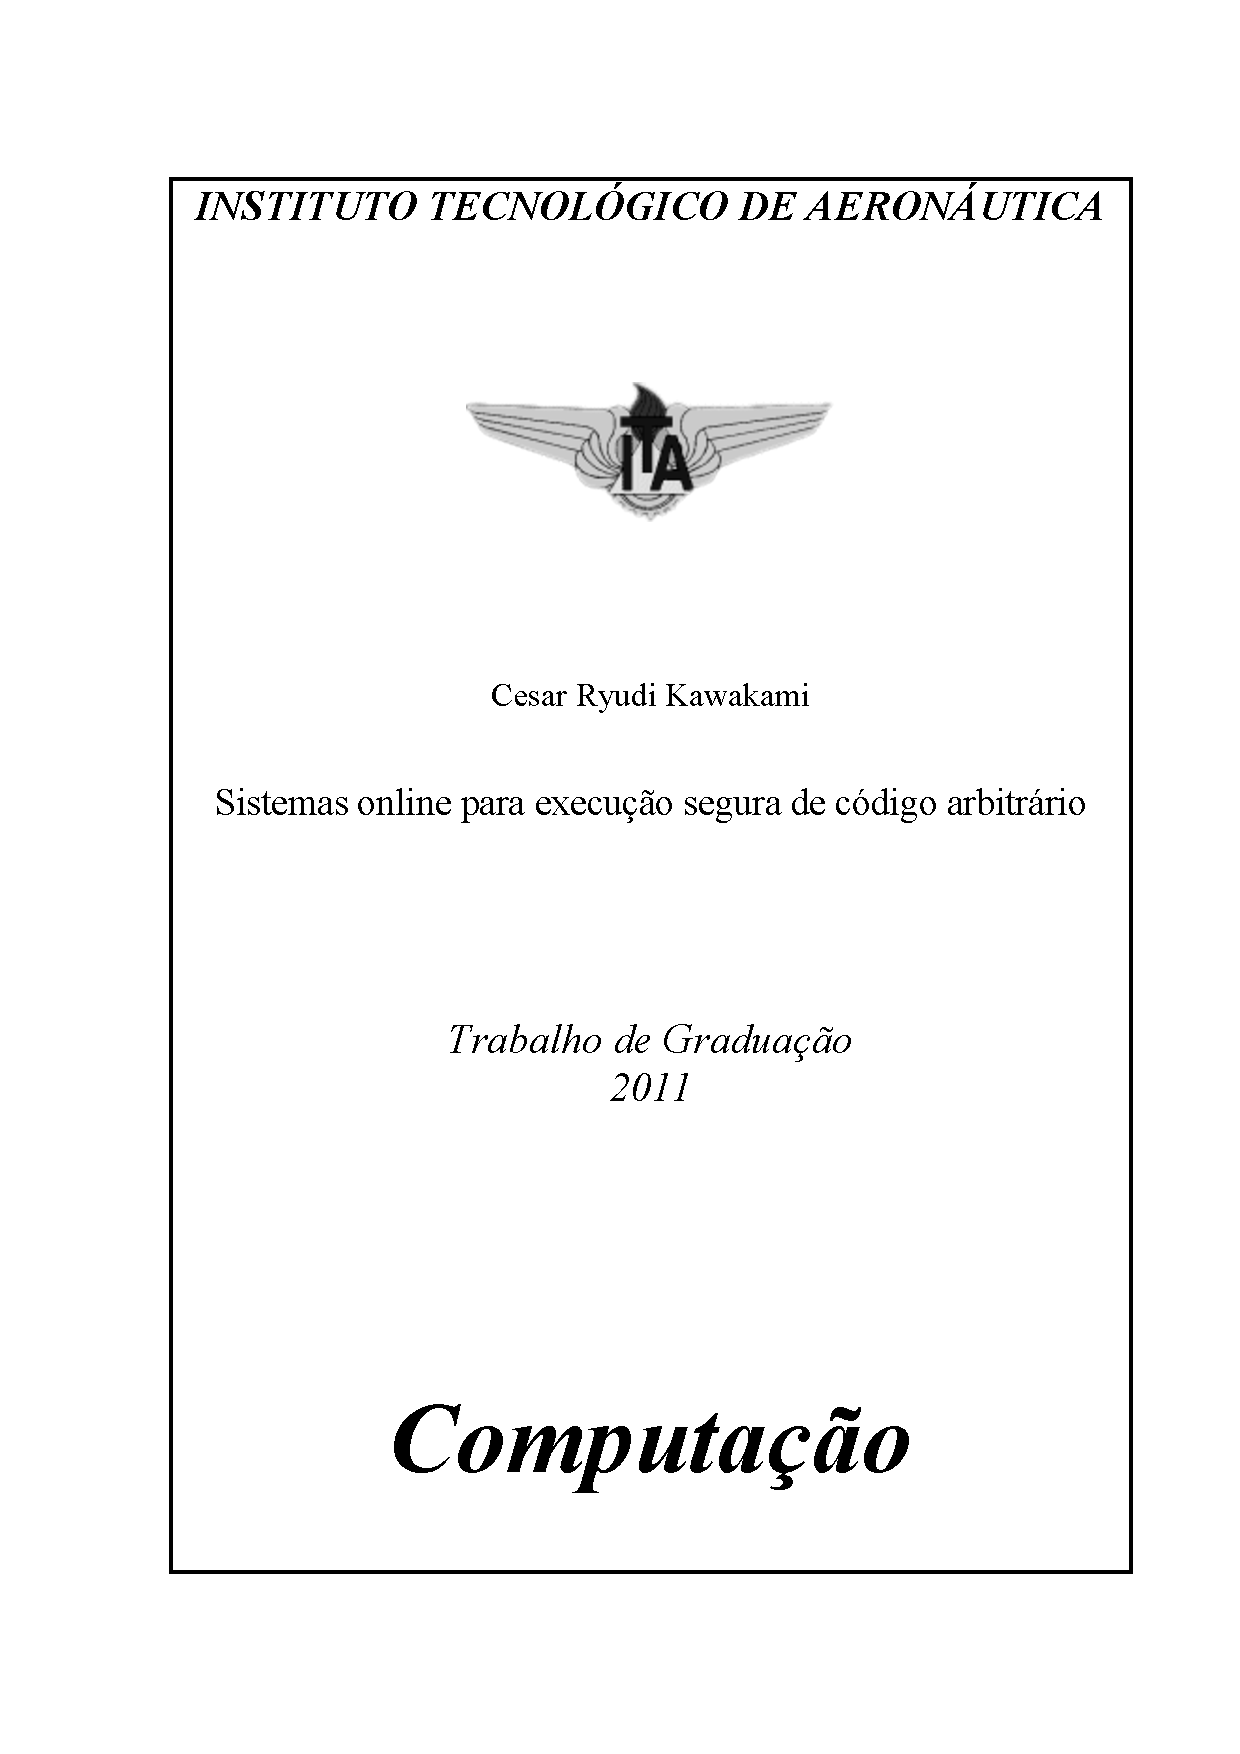
\includepdf{capa}

\pagenumbering{arabic}


\includepdf{rosto}

%\folhaderosto

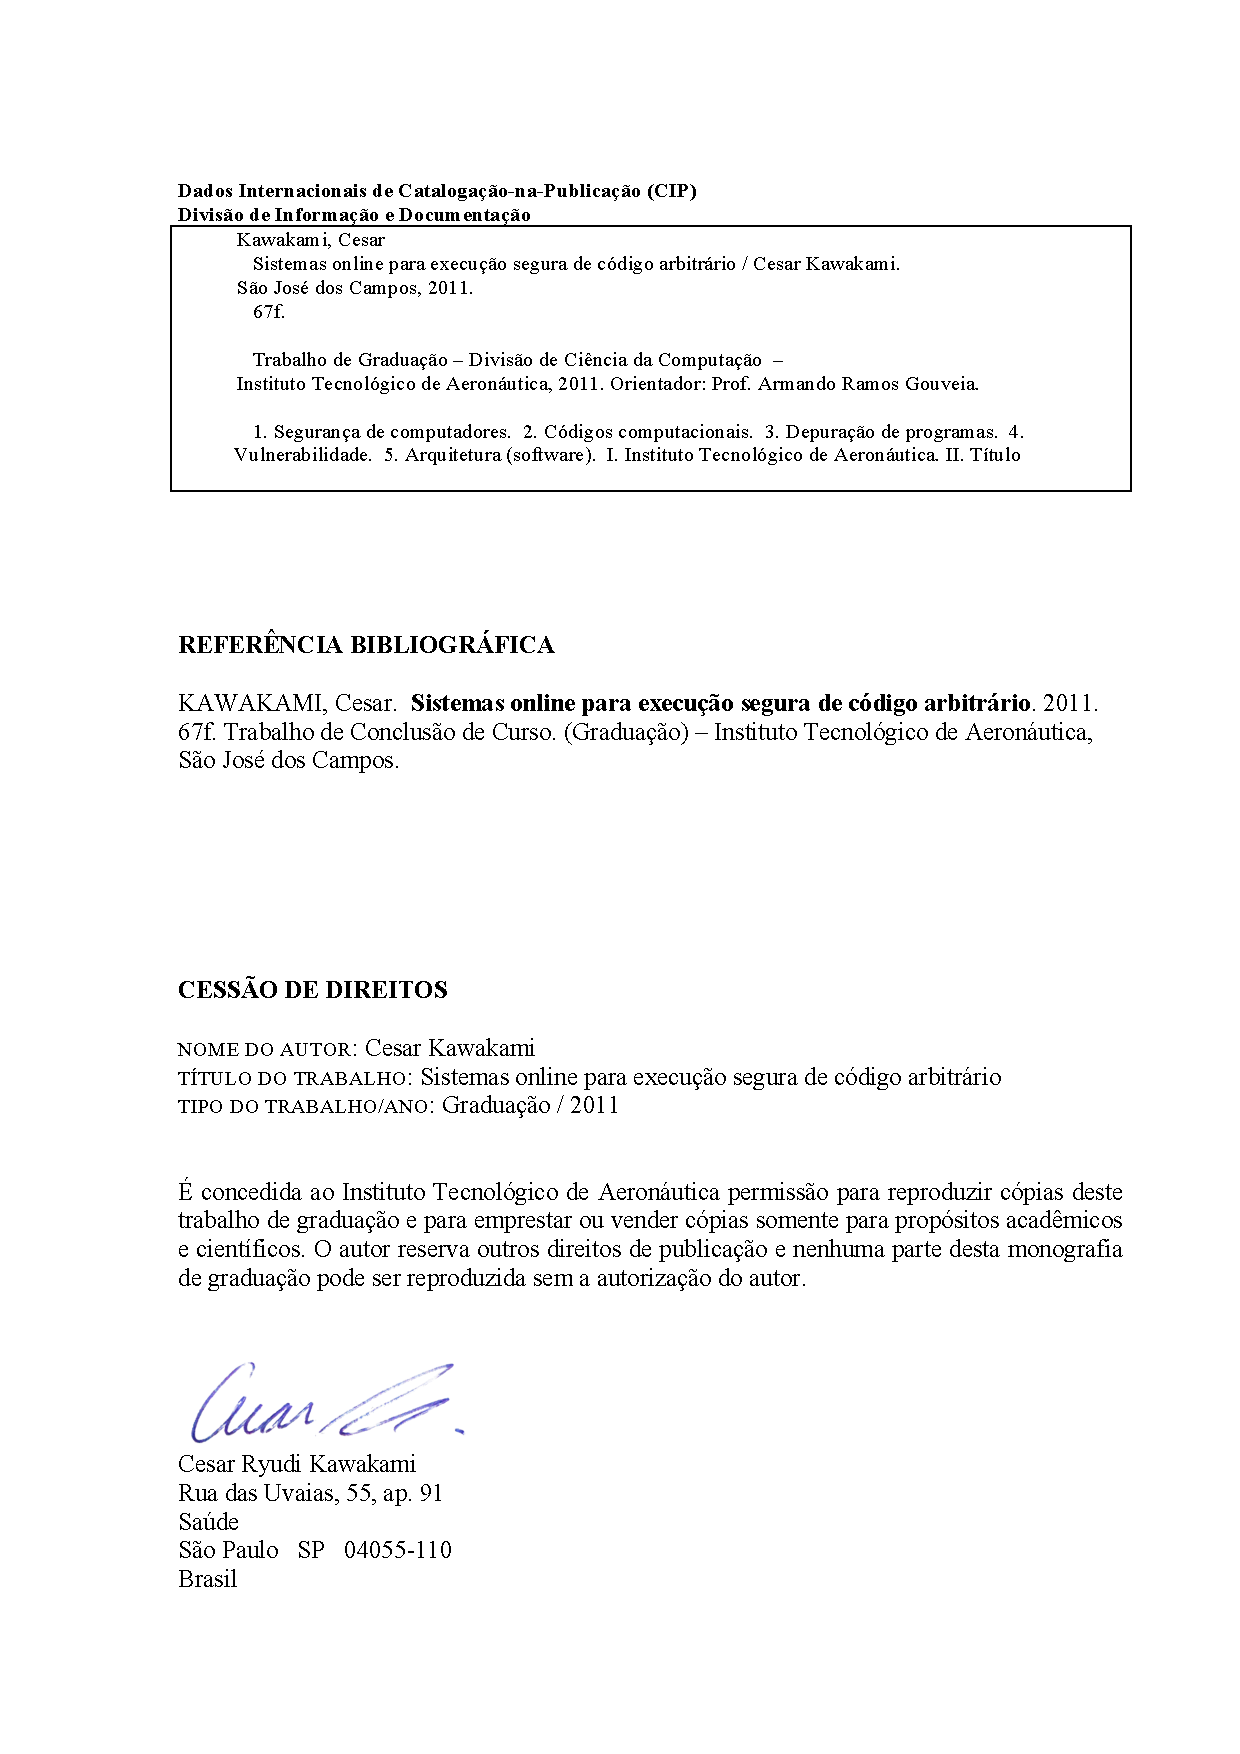
\includepdf{versorosto}

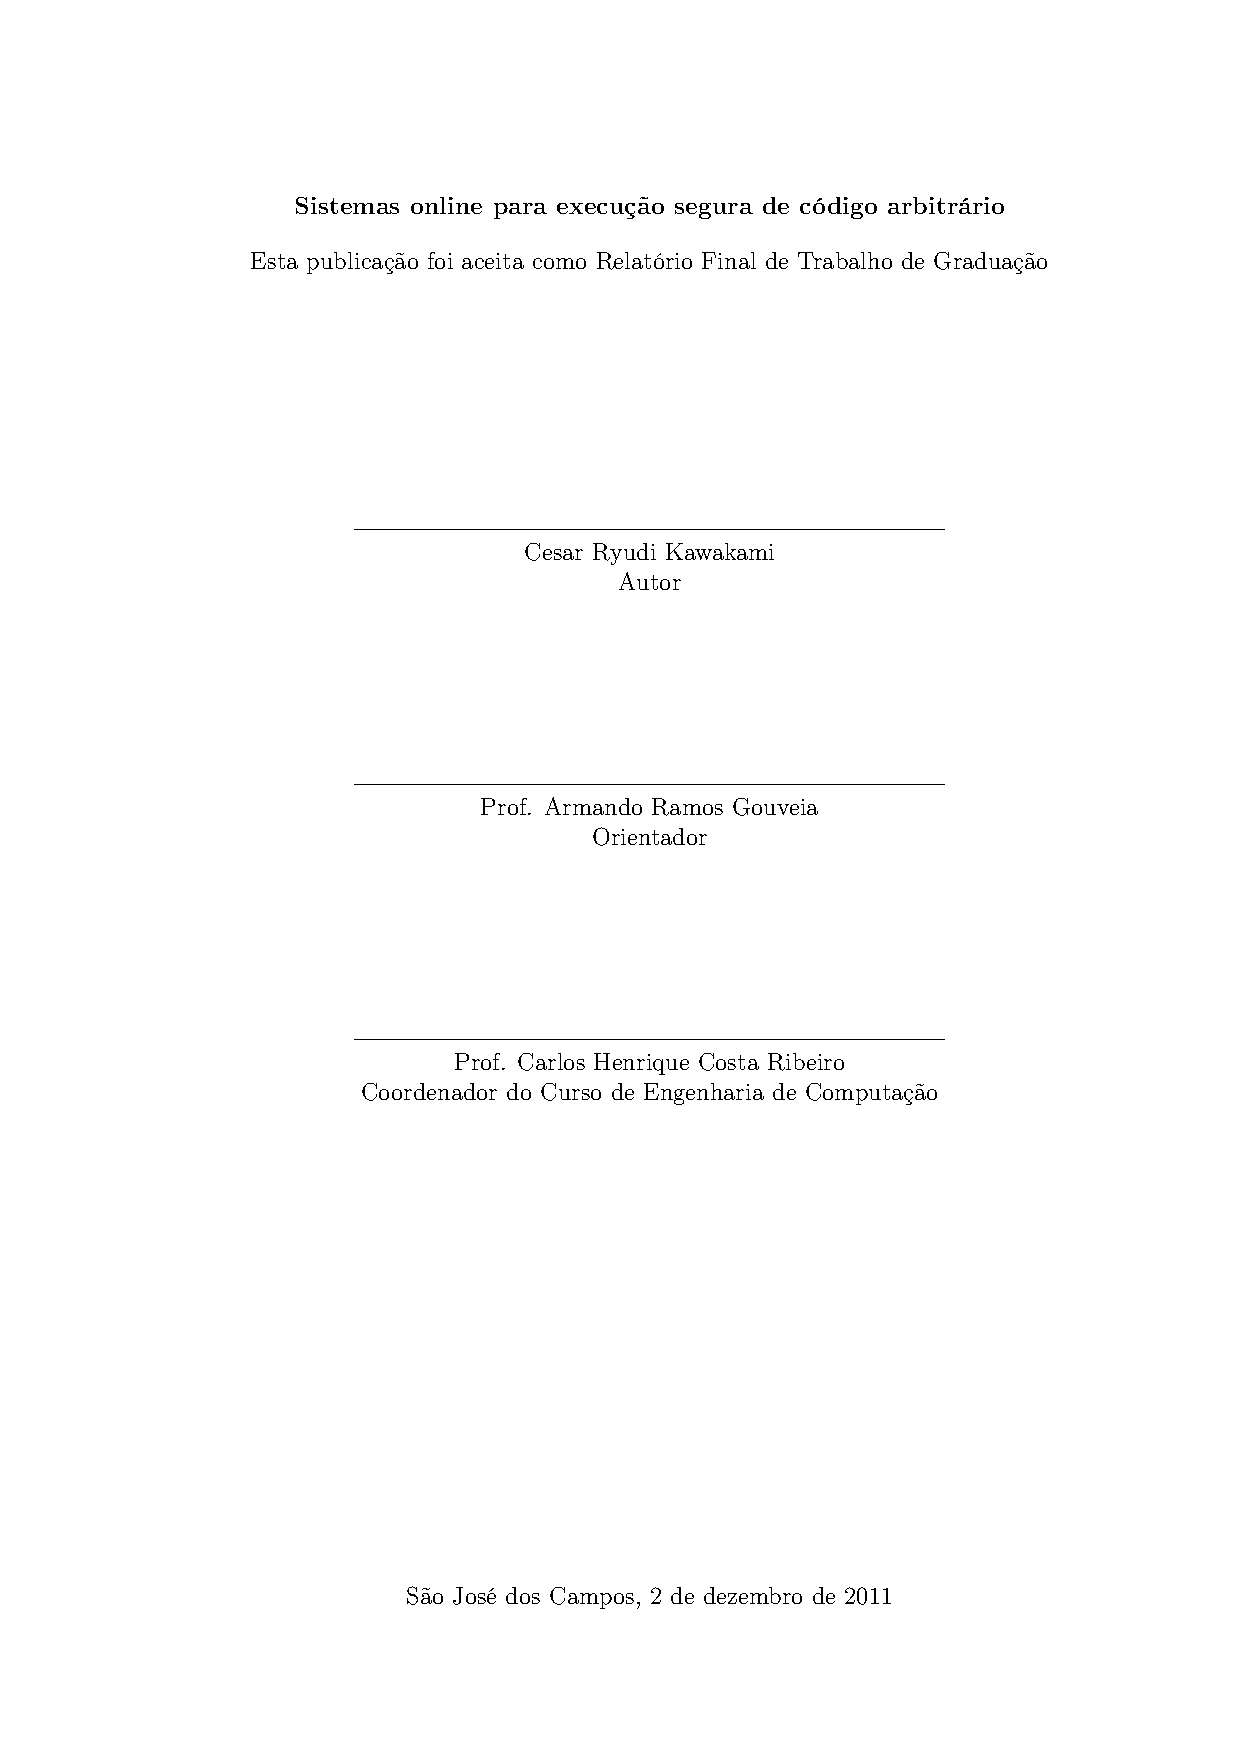
\includepdf{aprovacao}

%\begin{folhadeaprovacao}
%	\setlength\ABNTsignwidth{10cm}
%	\setlength\ABNTsignthickness{0.4pt}
%	\setlength\ABNTsignskip{3cm}
%	\begin{center}
%		\textbf{Sistemas online para execução segura de código arbitrário}
%		
%		Esta publicação foi aceita como Relatório Final de Trabalho de Graduação
%	\end{center}
%	\assinatura{Cesar Ryudi Kawakami \\ Autor}
%	
%	\assinatura{Prof. Armando Ramos Gouveia \\ Orientador}
%	
%	\assinatura{Prof. Carlos Henrique Costa Ribeiro \\ Coordenador do Curso de Engenharia de Computação}
%	\vfill
%	\begin{center}
%		São José dos Campos, 2 de dezembro de 2011
%	\end{center}
%\end{folhadeaprovacao}

\chapter*{}

\vfill

\begin{flushright}
A todos os meus amigos,\\
porque sobreviver ao ITA, acadêmica e pessoalmente, seria impossível sem vocês.
\end{flushright}

\vfill

\chapter*{Agradecimentos}

Os méritos deste trabalho merecem ser divididos com algumas pessoas.

Agradeço aos meus colegas de equipe na ACM ICPC, Guilherme Souza e Daniel Moreira, pela formação de uma equipe fantástica que possibilitou o conhecimento sobre competições de programação que serviu como uma das bases deste projeto.

Agradeço, também, ao Prof. Armando Gouveia, pessoa responsável pelas atividades do ITA na ICPC e também orientador deste trabalho. Sem seu esforço, a presença do ITA nas competições de programação talvez fosse muito menor e este trabalho talvez não fosse possível.

\begin{resumo}
Um sistema online para execução segura de código arbitrário é um sistema computacional voltado para a Internet que permita a execução segura de código proveniente de fontes não-confiáveis. A execução segura de código arbitrário é um tema pouco abordado na área de sistemas operacionais, uma vez que, em geral, assume-se que o usuário será o responsável pelos processos disparados. Os objetivos imediatos deste trabalho são fazer uma exposição dos casos de uso considerados para então elaborar uma arquitetura detalhada de um sistema que resolve o problema e montar um protótipo funcional. São estudadas duas aplicações: competições de programação, que avaliam os competidores executando seus códigos contra uma bateria secreta de testes, e as IDEs online, que permitem a execução de código sem necessitar da instalação de ambientes locais de desenvolvimento. Um levantamento é feito sobre os poucos sistemas já existentes que abordam os mesmos problemas. São descritas as principais tecnologias utilizadas e respectivas fundamentações teóricas durante o trabalho, incluindo Tornado, MongoDB, RabbitMQ, AppArmor e long polling. É apresentado o projeto de um sistema online para execução segura de código arbitrário. São descritas as considerações de design feitas, bem como as estratégias arquiteturais escolhidas, que incluem o uso de programação de alto nível, o uso de escalabilidade horizontal como meio para obtenção de performance e a segurança em profundidade. É apresentada a arquitetura do sistema, com uma exposição sobre a sua visão geral, bem como a arquitetura dos subsistemas, o modelo de segurança e os protocolos de comunicação. Finalmente, um protótipo funcional para cada um dos casos de uso estudados é mostrado, seguido de uma breve análise de validação. O protótipo apresentou-se performante, com escalabilidade horizontal linear e resistente aos ataques testados. No futuro, pode ser feito um aprofundamento sobre as possibilidades criadas por sistemas seguros para execução de código arbitrário, bem como sobre a problemática envolvida na elaboração de sistemas mais completos para o problema estudado.
\end{resumo}

\begin{abstract}
An online system for safe arbitrary code execution is a computational system for the Internet which allows for safe execution of code from unreliable sources. Works about safe execution of arbitrary code are rare in the literature since operating systems, in general, make the assumption that the user is well aware and trusts the processes running on the system. The immediate objectives of this work are to make an exposition of the use cases that are the focus of this work, then present a detailed architecture that solves the proposed problem, and build a functional prototype. Two main use cases are studied: programming competitions, which evaluate contestants by running their codes against a battery of secret test cases, and online IDEs, which allow running code without the user having to install any kind of local development environment. A brief survey is done regarding the few existing systems that solve the same kinds of problems. The main technologies that are used in this work are described together with some theoretical background, including Tornado, MongoDB, RabbitMQ, AppArmor and long polling. We then present a general framework for an online system for safe arbitrary code execution. The main design considerations are described, as well as the chosen architectural strategies which include the use of high-level programming, horizontal scalability as the path to greater performance and security in depth. The architecture of the proposed system is presented, including an overview, the architecture of each of the subsystems, the security model and the communication protocols. Finally, a functional prototype for each of the studied use cases is shown, followed by a brief validation analysis. The prototype performs well, showing linear horizontal scalability and resistance against a known list of attacks. In the future, more studies can be done regarding the possibilities created by safe online environments for executing arbitrary code, as well as the problems involved in designing more complete systems for the studied use cases.
\end{abstract}

\bookmark[level=0, page=1]{Capa}
\bookmark[level=0, page=2]{Folha de rosto}
\bookmark[level=0, page=3]{Verso da folha de rosto}
\bookmark[level=0, page=4]{Folha de aprovação}
\bookmark[level=0, page=5]{Dedicatória}
\bookmark[level=0, page=6]{Agradecimentos}
\bookmark[level=0, page=7]{Resumo}
\bookmark[level=0, page=8]{Abstract}
\bookmark[level=0, page=9]{Sumário}

\tableofcontents

\listoffigures

\listoftables

\lstlistoflistings

\renewcommand\nomname{Lista de Abreviaturas e Siglas}
\printnomenclature

\chapter{Considerações iniciais}

Neste capítulo inicial, são feitas considerações iniciais sobre a natureza deste trabalho de graduação, bem como sua motivação e o nicho em que se insere dentro da disciplina da engenharia de computação. Descreveremos o que são \emph{sistemas online para execução segura de código arbitrário} e as principais aplicações consideradas, as \emph{competições de programação} e os \emph{ambientes integrados de desenvolvimento online.} Explicaremos, então, as características que são esperadas dos sistemas em questão e faremos uma breve exposição dos sistemas e estudos já existentes na atualidade.

\section{Motivação}

\nomenclature{SESC}{Sistema online para execução segura de código arbitrário}

Um \emph{sistema online para execução segura de código arbitrário} (SESC) é um sistema computacional voltado para a Internet e que permita a execução segura de código proveniente de fontes não-confiáveis. Em geral, são sistemas que provêm o uso desse serviço diretamente ao usuário final, permitindo que este execute aplicações ou trechos de código e obtenha os resultados desta execução, mas delegue a responsabilidade da execução do código em si aos servidores de aplicação.

SESCs são sistemas interessantes e necessários a uma gama de aplicações. Entre as principais aplicações de sistemas desse tipo, encontram-se as competições de programação, como a International Olympiad in Informatics e a International Collegiate Programming Contest; e os ambientes integrados de desenvolvimento online, como o disponível no site \verb|http://www.ideone.com|. Em seções posteriores, examinaremos mais a fundo cada um desses casos de uso.

\section{Objetivos}

Este trabalho tem, por fim, analisar de maneira extensiva a problemática envolvida com o \emph{design} e a implementação de SESCs, bem como apresentar uma proposta de sistema que exibe as características desejadas e uma implementação prototípica das funcionalidades mais críticas aliada à sua validação.

\section{Estrutura do trabalho}

A fim de proporcionar uma divisão natural dos temas expostos neste trabalho e facilitar sua leitura, o texto foi dividido na seguinte sequência de capítulos.
\begin{itemize}
	\item O \emph{capítulo 2} expõe os casos de uso nos quais este trabalho se baseia, fazendo uma exposição do problema e uma análise das características que o sistema sob estudo deve apresentar. Ao final, é feito um levantamento do material existente sobre o tema.
	\item O \emph{capítulo 3} faz uma exposição das ferramentas e tecnologias abordadas e utilizadas ao longo do trabalho.
	\item O \emph{capítulo 4} apresenta o projeto de sistema central a este trabalho, fazendo uma análise extensiva das decisões de arquitetura envolvidas e uma exposição do protótipo de sistema final implementado.
	\item Finalmente, o \emph{capítulo 5} conclui o trabalho expondo as conclusões a que o autor chegou e comentários levantados ao longo do projeto.
\end{itemize}

\chapter{O problema}

Neste capítulo, faremos uma exposição dos principais casos de uso que foram levados em conta durante a realização deste trabalho. A seguir, faremos uma análise das principais características que um sistema online para execução segura de código arbitrário deve apresentar. Finalmente, exporemos um levantamento feito sobre quais sistemas existem na atualidade e procuram resolver a mesma classe de problemas.

\section{Competições de programação}

\nomenclature{ICPC}{International Collegiate Programming Contest}
\nomenclature{IOI}{International Olympiad in Informatics}
\nomenclature{GCJ}{Google Code Jam}

As competições de programação, como a \emph{International Olympiad in Informatics} (IOI) \cite{ioinformatics}, a ACM International Collegiate Programming Contest (ICPC) \cite{acmicpc} e a Google Code Jam (GCJ) \cite{googlecodejam}, são eventos de porte significativo com alcance mundial, posicionando-se como excelentes vetores de divulgação das ciências da computação, além de ensino, inspiração e captura de talentos nesse campo. Numa área do conhecimento de desenvolvimento ainda incipiente ao redor do mundo, tem-se um positivo número anual de mais de 100.000 participantes estudantis mundialmente \cite{icpcfactsheet,wang2010selection}.

O formato geral dessas competições consiste na resolução de um certo número de situações-problema (em geral, de três a doze) em um determinado intervalo de tempo, usualmente de cinco horas. A resolução de um problema, neste caso, compreende a interpretação da situação, a elaboração de uma estratégia de solução viável nos termos das restrições da situação e a correta implementação dessa solução em uma linguagem de propósito geral como C/C++, Pascal ou Java. As soluções em prova são avaliadas unicamente pela correção e eficiência de sua implementação. 

Restrições, dados e entradas dos problemas são desenhados de maneira a possibilitar a correção automatizada das soluções dos competidores, que são executadas em servidores contra uma bateria de entradas elaboradas pela banca examinadora a fim de determinar (julgar) a pontuação do competidor para aquele problema. Em competições no formato da ICPC, as soluções dos competidores são julgadas assim que recebidas de modo fornecer realimentação o mais rápido possível.

Embora cada competição empregue condições diferentes de aceitação e graduação das soluções enviadas, são dois os principais critérios utilizados. Os programas são avaliados pela sua \emph{correção} através da comparação dos resultados emitidos contra um catálogo de entradas e saídas esperadas elaborado pela comissão julgadora. Os programas são também avaliados pela sua \emph{eficiência} através do seu tempo de execução total em relação à bateria de testes executada, para a qual existe um tempo-referência máximo. Tais tempos-referência baseiam-se nas melhores soluções conhecidas para o problema em questão implementadas pela banca, e a configuração do problema é ajustada para se ter tempos máximos no entorno entre alguns segundos e alguns minutos.

Em competições de estilo ICPC, os resultados das análise das soluções submetidas são fornecidos assim que disponíveis durante a competição, usualmente após poucos minutos. Tal realimentação permite à equipe mal sucedida modificar sua solução para tentar corrigir o problema. A fim de manter o desafio, porém, apenas um conjunto enxuto de sinais é enviado aos competidores, geralmente composto de 4 sinais, nomeadamente:
\begin{itemize}
	\item \emph{Accepted,} para soluções aceitas como corretas pelo sistema.
	\item \emph{Wrong answer,} para soluções tidas como incorretas pelo sistema através da análise da saída do programa.
	\item \emph{Time limit exceeded,} para soluções tidas como ineficientes pelo sistema por terem excedido o tempo-referência máximo para o problema.
	\item \emph{Runtime error,} para soluções tidas como incorretas pelo sistema por terem encontrado um erro durante sua execução.
\end{itemize}

Devido à elevada relação número de problemas--tempo disponível, ficando em menos de 30 minutos por problema em competições como a ICPC, são provas em que o tempo é considerado recurso escasso e de controle essencial para uma boa eficiência.

\clearpage
\section{Ambientes integrados de desenvolvimento online}

\nomenclature{AIDO}{Ambiente Integrado de Desenvolvimento Online}

Outra aplicação interessante e de importância de SESCs são os \emph{Ambientes Integrados de Desenvolvimento Online} (AIDO). AIDOs são sistemas online que permitem ao usuário editar e ver o resultado da execução de seu código diretamente via internet, sem uso de ferramenta externa que não seu navegador. Entre os exemplos proeminentes de AIDOs encontram-se o IDEOne \cite{ideoneabout} e o Codepad \cite{codepadabout} \figref{codepad}.

\fig{codepad}{Tela principal do aplicativo Codepad}

No caso de uso principal, o usuário abre a página do AIDO, escreve ou cola o código a ser testado, efetua o envio e, logo depois, já tem acesso aos resultados de seu programa compilado. A agilidade e facilidade de uso desses sistemas abre possibilidades no campo do desenvolvimento de software:
\begin{itemize}
	\item No \emph{aprendizado de linguagens de programação}, a barreira de entrada diminui drasticamente, uma vez que o aluno não mais tem de despender recursos para configurar seu próprio ambiente de desenvolvimento, optando por um ambiente online que está constantemente disponível. Além disso, a interface dos AIDOs é, em geral, muito mais simples do que suas contrapartes locais nas máquinas dos alunos, permitindo aos alunos focar no aprendizado da linguagem em si, e não da parafernalha necessária para permitir a execução do código.
	
	\item Os AIDOs também permitem um \emph{desenvolvimento colaborativo e remoto de software} de maneira altamente conveniente, permitindo que a comunicação entre as partes ocorra de maneira eficiente. A execução online de código permite às partes colaborar sobre o desenvolvimento sem, necessariamente, deixar o ambiente do \emph{browser} para utilizar algum \emph{software} dedicado.
\end{itemize}

Sob o ponto de vista computacional, sistemas informatizados para competições de programação e AIDOs apresentam grande interseção de características, sendo ultimamente duas aplicações de SESCs. Neste trabalho, os SESCs, seus requisitos e suas características serão abordados sob um ponto de vista mais amplo, englobando tanto as necessidades de competições de programação quanto de AIDOs.

\section{Características esperadas}

As competições de programação e os ambientes integrados de desenvolvimento online são dois casos de uso que exibem, para sua boa condução, um conjunto de requisitos peculiar. Sistemas informatizados específicos tornam-se, então, ferramentas de fundamental importância. Entre as características necessárias a um bom SESC voltado às aplicações em questão, podem ser ressaltados os seguintes pontos.

\subsection{Escalabilidade}

No contexto das competições de programação, devem ser considerados cenários de provas \emph{on-site}\footnote{Situações em que todos os competidores competem em um mesmo local designado.} com mais de 500 clientes como durante a IOI \cite{ioi-nl1-2007} e provas \emph{off-site}\footnote{Situações em que a prova é praticada inteiramente através da internet, assim atingindo escala mundial facilmente.} com mais de 30.000 clientes simultaneamente como durante a GCJ \cite{googlecodejamhistory}. Ao mesmo tempo, AIDOs são, em geral, sistemas voltados para o uso da comunidade em geral, podendo requerer uma quantidade bastante significativa de recursos. Considerando o padrão de uso pesado dos sistemas envolvidos, particularmente devido ao requerimento de executar por um intervalo de tempo não-trivial pedaços de código arbitrário enviados pelos usuários, surge a necessidade de boa \emph{escalabilidade} do sistema, em especial no sistema de execução de código arbitrário.

A \emph{escalabilidade} de um sistema, sob o ponto de vista da computação, é a sua habilidade de lidar com o crescimento de sua demanda. Sistemas escaláveis apresentam arquiteturas que podem ser expandidas conforme a demanda cresce, e cujo custo dessa expansão não se torna proibitivo quando comparados aos respectivos ganhos em demanda.

Sistemas online para execução de código arbitrário, devido aos altos requisitos que apresentam em termos de poder computacional, devem então levar em conta a devida escalabilidade de suas arquiteturas. Eventuais crescimentos de demanda, tanto em competições de programação quanto em AIDOs, são totalmente plausíveis, e qualquer SESC devidamente planejado deve administrar tal crescimento em demanda de maneira de maneira elegante.

\subsection{Resposta rápida e comunicação bidirecional}

As competições de programação são provas em que o tempo é escasso e grande parte das interações depende do sistema em questão. Visando uma boa condução da competição, o sistema deve buscar exigir do usuário interação e espera mínimas para operação. Um sistema pouco ergonômico causa atrasos que se acumulam ao longo do tempo de uma prova.

A título de exemplo, numa competição estilo ICPC, considere-se uma prova com 5 horas de para a resolução de 10 problemas. Tomando por base um número médio de 4 tentativas por problema, devem ser consideradas 40 submissões. Se cada submissão tomar do competidor 1 minuto, terão sido gastos, ao final da prova, um total de 40 minutos (comparados às 5 horas disponíveis) apenas em interações com um sistema que deveria ser transparente à situação.

Ainda no âmbito da eficiência na interface do sistema e novamente considerando as características do problema, é necessário ao competidor um acompanhamento em ``tempo real'' do andamento da prova e dos outros competidores. Em divergência da grande maioria dos sistemas web remotos da atualidade, surge a necessidade de comunicação bidirecional na qual, além do quadro comum em que o cliente requisita informações do servidor, seja possível, também, o quadro em que o servidor, munido de nova informação, a ``empurra'' para os clientes sem que haja necessidade de requisição.

A arquitetura da internet da atualidade não foi desenhada para este caso de uso, e a problemática consequente é analisada posteriormente neste trabalho.

\subsection{Segurança da informação}

Qualquer sistema operacional exposto a uma quantidade não-trivial de usuários desconhecidos apresenta alta exposição aos riscos de \emph{segurança da informação.} O problema é ainda mais significativo durante as competições de programação, considerando sua alta importância e a natureza secreta dos dados em questão durante a competição em si.

No contexto da segurança da informação, é utilizado como base o triângulo composto por confidencialidade, integridade e disponibilidade \cite{stamp2011}. A \emph{confidencialidade} se trata do princípio pelo qual o acesso a informações deve ser negado ou impedido de alguma forma às partes que não foram autorizadas para tal. A \emph{integridade} trata da prevenção~--- ou, em último caso, detecção~--- de alterações ou deleções dos dados existentes por partes não autorizadas. Finalmente, com a crescente preocupação com ataques de negação de serviço através da internet, a \emph{disponibilidade} dos sistemas passou a ser preocupação fundamental no desenho de sistemas focado em segurança da informação.

Devido à característica peculiar de execução de código arbitrário, os sistemas em questão são particularmente suscetíveis a uma ampla gama de ataques \cite{tochev2010,forisek2006security}. As seguintes categorias de ataques destacam-se como de particular relevância.
\begin{itemize}
	\nomenclature{DoS}{Denial of Service}
	\item Ataques de \emph{negação de serviço} (DoS, do inglês \emph{denial of service}) visam afetar a disponibilidade do sistema alvo, e são preocupação inerente a qualquer sistema informatizado, em particular aqueles com envolvimento da web. AIDOs, que apresentam em sua natureza a exposição à comunidade em geral, são particularmente suscetíveis a este tipo de ataque.
	
	\item Ataques de \emph{escalação de privilégios} são usualmente considerados um segundo passo após um bem-sucedido ataque de execução de código arbitrário. No contexto de SESCs, esta primeira ``porta'' já se encontra aberta, tornando a análise dos potenciais ataques de escalação de privilégios crucial, afetando os três componentes da segurança da informação.
	
	\item Ataques \emph{destrutivos} podem ser considerados versões mais graves de ataques de disponibilidade, buscando a desconstrução de funcionalidades do sistema ou de suas medidas de segurança a fim de afetar a integridade ou a disponibilidade do sistema informatizado. Ataques destrutivos são também facilitados pela característica aberta quanto à execução de código externo dos sistemas em questão.
	
	\item Ataques por \emph{canal dissimulado (covert channel)} atuam pela utilização, pelo atacante, de meios não previstos ou intencionados pelo arquiteto do sistema para comunicar informação. No contexto geral, são geralmente utilizados para a transmissão de informação confidencial à usuários ou áreas não autorizadas, e sua importância no âmbito das competições de programação se dá da mesma maneira. A título de exemplo, um programa poderia fornecer informações confidenciais sobre os casos de teste a que está sendo exposto fazendo uso da emissão de sinais de realimentação que são retornados pelo sistema ao competidor automaticamente.
\end{itemize}

Qualquer sistema \emph{online} que possibilite a execução de código arbitrário encontra-se altamente exposto a cada um dos itens acima, e deve levar em consideração um cuidado peculiar no desenho de sua arquitetura de segurança.

\section{Sistemas já existentes}

Além do IDEOne e do Codepad já citados, faremos uma breve apresentação dos SESCs de destaque na atualidade.

\begin{itemize}
	\nomenclature{BOCA}{Boca Online Contest Administrator}
	\item O \emph{Boca Online Contest Administrator} (BOCA) é um sistema brasileiro \cite{boca2004} de apoio a competições de programação desenvolvido para ser usado na Maratona de Programação da Sociedade Brasileira de Computação. É utilizado principalmente nas competições brasileiras de programação para estudantes universitários em níveis local e nacional, onde ocorre a troca de conhecimentos que facilita o uso desse sistema. Trata-se de um sistema já testado em um significativo número de competições, oferecendo a opção de julgamento automático de submissões. O sistema não possui garante por si a segurança do sistema, deixando a cargo do administrador a tomada das precauções necessárias.
	
	\item O \emph{Mooshak} \cite{mooshak2003} é um sistema baseado em Web para a administração e correção de competições de programação. É utilizado principalmente no noroeste da Europa, sendo o sistema de preferência na prova regional-noroeste da ICPC europeia. A interface do Mooshak não acontece via navegador, necessitando de um aplicativo cliente específico para o acesso ao sistema.
	
	\item O \emph{KATTIS} \cite{kattis2011} é um sistema voltado para o ensino de programação, focando seu caso de uso principal na avaliação e correção automatizada para uso em tarefas relacionadas a cursos de programação. Ainda assim, sua robustez o leva a ser utilizado em competições de grande porte, como a fase final mundial da ACM ICPC. Sua difusão é limitada por ser um sistema de código fechado, necessitando a contratação de terceiras partes para implementação e treinamento dos usuários do sistema.
\end{itemize}

Devido a, em geral, SESCs serem considerados uma aplicação de nicho, a literatura não demonstra uma variedade muito grande de sistemas disponíveis para utilização e estudo. São poucos os sistemas projetados para uso geral e aberto ao público; sendo assim, a grande maioria dos SESCs apresenta-se oculta ao conhecimento aberto, provavelmente como uma maneira de obter segurança por obscuridade.

\chapter{Tecnologias utilizadas e fundamentação teórica}

Neste capítulo, faremos uma exposição das ferramentas e das tecnologias abordadas e utilizadas ao longo deste trabalho, bem como uma breve apresentação dos principais fundamentos teóricos relacionados a cada ferramenta. Nas seções seguintes, analisaremos:
\begin{itemize}
	\item O \emph{Tornado,} um \emph{framework} escalável \emph{web} em Python;
	\item O \emph{MongoDB,} um banco de dados de alta performance orientado a documentos;
	\item O \emph{RabbitMQ,} um \emph{middleware} orientado a mensagens para computação distribuída;
	\item O \emph{AppArmor,} um sistema de controle de acesso obrigatório para \emph{kernels} Linux;
	\item O \emph{long polling,} uma técnica que permite o desenvolvimento de aplicações com comunicação \emph{push} num meio tradicionalmente \emph{pull} como a \emph{web.}
\end{itemize}

Muitas das tecnologias apresentadas são bastante modernas e não dispõem de boa documentação sobre seu funcionamento interno. Neste trabalho, quando possível, fez-se esforço pela elaboração de textos e diagramas que expliquem na medida do razoável os tópicos de maior importância referentes a cada ferramenta.
	
\section{Tornado}

O \emph{Tornado} é um \emph{framework} de aplicações \emph{web} desenvolvido em Python, bem como um servidor \emph{web} integrado. O Tornado é um servidor notado pela sua alta performance \cite{tornado2009}, sendo cerca de quatro vezes mais rápido do que aplicações similares desenvolvidas na mesma linguagem. O framework é também conhecido pela sua abordagem na solução do chamado ``problema das 10 mil conexões.''\footnote{O ``problema das 10 mil conexões'' refere-se à dificuldade de otimizar servidores \emph{web} para saber administrar com eficiência um algo número de clientes simultaneamente. O nome surge do número estimado máximo que essa classe de servidores atende, girando em torno de 10 mil.}

\nomenclature{E/S}{Entrada e saída (de dados)}

Para administrar um grande número de conexões simultaneamente, o Tornado utiliza uma abordagem chamada \emph{assíncrona.} Esta se dá em contraste com a abordagem \emph{síncrona,} considerada a tradicional no desenvolvimento de servidores em geral.

\subsection{Servidores com E/S síncrona}

Servidores \emph{web} tradicionais, como o Apache em sua implementação usual, fazem uso de uma abordagem \emph{síncrona,} ou seja, comandos de \emph{entrada e saída} (E/S) interrompem a execução do programa até o término do comando, impedindo a aplicação de, por exemplo, atender a outras requisições de clientes. Programas desenhados desta maneira obtém paralelismo através do uso de múltiplas \emph{threads} administradas pelo sistema operacional \figref{multithreaded-webservers}. Cada conexão iniciada dispara uma nova \emph{thread} e, assim, o servidor passa a ser capaz de atender a mais de uma requisição simultaneamente.

\figcustom{multithreaded-webservers}{Servidores \emph{web} síncronos com paralelismo por \emph{multithreading}}{bp}{.9}

Essa abordagem apresenta um grave problema de escalabilidade: os sistemas operacionais, por \emph{design,} apresentam um custo relativamente grande associado a cada \emph{troca de contexto\footnote{Situação em que uma thread tem sua execução interrompida para ceder seu tempo de CPU para outra. O ato de interromper a execução também é conhecido como \emph{preempção.}},} uma vez que oferecem uma série de garantias a cada \emph{thread,} como, por exemplo, isolamento das demais \emph{threads} executando no sistema. A criação em massa de \emph{threads} causada pelos servidores em questão, em conjunto com os custos computacionais envolvidos na administração de múltiplas threads, sobrecarrega o sistema, chegando a uma situação na qual gasta-se mais tempo de CPU em trocas de contexto do que executando as tarefas em si.

\subsection{A E/S assíncrona do Tornado}

Na abordagem \emph{assíncrona} adotada pelo Tornado, uma mesma \emph{thread} é capaz de atender diversos clientes simultaneamente. Neste caso, uma estrutura de código, chamada \emph{IO loop} \figref{tornado-ioloop} administra o atendimento das requisições, encaminhando cada nova requisição a uma nova instância do código de atendimento.

\fig{tornado-ioloop}{Diagrama de fluxo do atendimento de uma requisição em Tornado}

A cada requisição de E/S, o código de atendimento \emph{cede,} num paradigma muito semelhante ao multithreading cooperativo, o controle ao \emph{IO loop,} que retornará o controle ao atendimento quando a operação de E/S estiver concluída. Para isso, o código de atendimento, ao ceder, envia também ao IO loop uma função de \emph{callback,} que será chamada quando a requisição de E/S estiver terminada. Observe que todo o processo ocorre sem troca excessiva de dados e dentro de um único processo.

A abordagem adotada torna o atendimento de uma requisição uma operação muito leve, sendo que o programa inteiro é executado em apenas uma \emph{thread} do sistema operacional, causando uma diminuição significativa dos recursos consumidos quando comparada com uma implementação por \emph{threads.} Além disso, o servidor torna-se mais escalável, restringindo o sistema apenas às capacidades do computador em si, e não dos limites de processamento de threads do sistema operacional~--- em outras palavras, aumenta-se a escalabilidade vertical dos servidores. O servidor e framework Tornado é o sistema de escolha para a implementação deste projeto.

\section{MongoDB}

O \emph{MongoDB} é um sistema de banco de dados de alta performance e orientado a documentos. O sistema é notado por possuir alta escalabilidade e facilidade de uso, sendo utilizado em ambientes de produção em sites como Disney, Craigslist e MTV Networks.

O \emph{design} orientado a documentos utilizado pelo MongoDB possibilita alta performance e escalabilidade a um baixo custo. Bancos de dados orientados a documentos são servidores desenhados para o armazenamento, obtenção e administração de dados semi-estruturados, e são a principal categoria de banco de dados dentro dos chamados \emph{NoSQL,} uma nova geração de sistemas que se desprendem do paradigma relacional.

\subsection{Bancos de dados relacionais}

No paradigma relacional, um banco de dados se constitui por uma coleção de relações, frequentemente chamadas de tabelas. Cada tabela armazena informações sobre uma estrutura fixa, contendo sempre a mesma estrutura de dados~--- em geral, é tarefa difícil executar a alteração da estrutura de uma relação. O modelamento dos dados armazenados usualmente se faz por meio da chamada \emph{normalização,} na qual eliminam-se relações que não são fundamentalmente simples, quebrando-as em relações mais simples, além de qualquer redundância nos dados. Tal modelamento não faz uso das características em uso da aplicação, dependendo apenas dos dados a serem armazenados.

A título de exemplo, para o armazenamento do inventário de uma loja de artigos esportivos, poderíamos ter a relação \emph{modelo,} que referenciaria a relação \emph{marca} (uma marca pode ter vários modelos, mas um modelo tem apenas uma marca), e teríamos também a relação \emph{item} (um modelo pode ter vários itens, de diferentes cores, por exemplo, mas cada item é de apenas um modelo). Neste modelo, a recuperação de dados completos de um modelo, por exemplo, separados em várias relações, se faz através do uso dos chamados \emph{joins,} operações que associam relações, ``montam'' e retornam ao cliente uma estrutura completa.

O problema surge quando se deseja escalar horizontalmente os bancos de dados relacionais a um número significativo de servidores. Devido ao desconhecimento dos padrões de uso das aplicações por parte do modelo, a escalabilidade horizontal dos bancos de dados relacionais se dá através do \emph{estilhaçamento} dos dados de cada relação, no qual, de acordo com um critério de aleatoriedade ou que garanta a igualdade, os dados de uma relação são distribuídos entre os diversos servidores de bancos de dados. Por exemplo, enquanto os dados do modelo X podem estar no servidor A, os dados dos itens Y e Z (ambos do modelo X) podem estar nos servidores B e C, todos distintos. Isso torna as operações de \emph{join} significativamente mais complexas, envolvendo diversos servidores com uma troca aparentemente desordenada e muito custosa de informações.

Um percalço ainda maior surge quando são consideradas alterações aos bancos de dados. Devido à natureza espalhada que os dados adquirem quando normalizados (que os colocam em diversas relações) e estilhaçados (que colocam os elementos de cada relação em diversos servidores), as alterações, a fim de preservar a consistência dos dados, são usualmente encapsuladas em \emph{transações}~--- conjuntos de operações que, em grupo, preservam as características de \emph{atomicidade,} \emph{consistência,} \emph{isolamento} e \emph{durabilidade} que são as características essenciais de qualquer banco de dados. A questão é que transações em sistemas distribuídos são obrigadas a sincronizar (travar) recursos em todas as máquinas afetadas, diminuindo drasticamente a performance do sistema: um conjunto de máquinas atuando em sincronia age, efetivamente, na velocidade de uma única máquina.

Atendo-se aos sistemas relacionais, a solução usualmente adotada passa pela chamada \emph{denormalização} dos dados, que essencialmente procura aglomerar na mesma relação aqueles dados que costumem ser lidos e escritos de maneira conjunta na aplicação. A aplicação do inventário de artigos esportivos poderia, por exemplo, manter já na relação de modelo todas as informações referentes à marca e a cada um dos itens. Desta maneira, diminui-se a necessidade tanto de \emph{joins} quanto de transações distribuídas, possibilitando uma maior escalabilidade horizontal de tais sistemas. No entanto, tal abordagem foge da filosofia original de desenho de tais bancos de dados, o que apresenta desafios significativos; as relações de bancos de dados relacionais não foram desenhadas para suportar alterações estruturais com facilidade. Além disso, perde-se a maioria das vantagens apresentadas pelos bancos de dados relacionais, como o forte estruturamento dos dados armazenados.

\subsection{Bancos de dados orientados a documento}

Os chamados bancos de dados \emph{orientados a documento} são uma classe de bancos de dados desenhados para o armazenamento de dados semi-estruturados. Fazem parte de uma variedade mais ampla chamada  \emph{NoSQL\footnote{Algumas vezes expandido como ``not only SQL''.}} que se baseia em paradigmas diferentes do clássico modelo relacional. Seu destaque no cenário atual se dá pelo fato de que, de maneira geral, as escolhas de design que guiam tais bancos de dados são focadas na manutenção de características específicas dos bancos de dados relacionais, enquanto outras são descartadas em favor da escalabilidade horizontal.

Dentro da classe dos \emph{NoSQL,} destacam-se os bancos de dados orientados a \emph{documento.} Como implicado pelo nome, tais bancos de dados são desenvolvidos em torno da noção de \emph{documento,} uma porção estruturada de dados razoavelmente completa. Os documentos são, de certa forma, similares ao conceito de registros nos bancos de dados relacionais, mas são muito menos rígidos. Principalmente, os documentos não são obrigados a aderir uma esquema determinado, ou seja, não são obrigados a conter as mesmas classes de informações (que seriam consideradas colunas no modelo relacional).

De maneira geral, os documentos são endereçados no banco de dados através de um identificador único, em paralelo ao conceito de chave primária no modelo relacional. Sendo assim, o acesso aos documentos pode ser realizado através desse identificador único. Por outro lado, uma das funcionalidades características do modelo orientado a documento é a capacidade de realizar buscas e demais operações sobre os documentos com base nos conteúdos dos mesmos, ainda que seus conteúdos não ofereçam, todos, a mesma estrutura. Neste caso, o modelo orientado a documento equipara o modelo relacional no poder de busca, se não o ultrapassa.

O efetivo uso dos bancos de dados orientados a documento requer o correto uso do \emph{modelamento orientado a documento,} que se distancia de maneira razoável do paradigma relacional. De maneira geral, relacionamentos entre entidades do tipo ``contém-um,'' como a relação entre uma uma mão e as cartas que possui, são modelados por \emph{embutimento,} ou seja, as cartas são, todas, colocadas diretamente no documento que corresponde à mão. Enquanto tal abordagem causa redundâncias no banco de dados, torna muito mais rápido o acesso se o caso de uso mais comum seja o acesso à mão como um todo ao invés de cada carta individual. Nas aplicações práticas, a grande maioria dos acessos a bancos de dados se caracteriza por este padrão aglomerado.

Devido ao aglomeramento de informações relacionadas e consequente ausência da necessidade de \emph{joins,} bancos de dados orientados a documento podem ser escalados horizontalmente a um número significativamente grande de servidores. No caso específico do MongoDB, a escalabilidade se dá, novamente, através do estilhaçamento dos dados~--- porém, agora, como os componentes de cada informação não se encontram espalhados entre vários servidores, cada requisição atinge apenas um servidor, fazendo o que o sistema reaja quase linearmente ao aumento no número de servidores, numa performance quase ótima.

Como maneira de possibilitar uma maior escalabilidade horizontal do sistema, os bancos de dados orientados a documento e, entre eles, o MongoDB, são as opções de escolha na implementação deste trabalho.

\section{RabbitMQ}

O \emph{RabbitMQ} trata-se de um software de \emph{message-oriented middleware,} uma infra-estrutura de comunicação entre componentes de software dentro de um sistema distribuído. Um message-oriented middleware age como uma base e como um \emph{framework} para o desenvolvimento de sistemas distribuídos, abstraindo os detalhes da implementação da transferência de mensagens, seu encaminhamento e enfileiramento, bem como as idiosincrasias de cada plataforma, linguagem e sistema operacional envolvidos.

\nomenclature{AMQP}{Advanced Message Queuing Protocol}

O RabbitMQ implementa o protocolo \emph{Advanced Message Queuing Protocol} (AMQP) de troca de mensagens, e suporta diversos padrões de troca de mensagens distribuída. Os principais padrões de troca de mensagens serão explicitados a seguir.

\subsection{Troca de mensagens por distribuição de tarefas}

No padrão de \emph{distribuição de tarefas} \figref{rabbitmq-workqueue}, também conhecido como \emph{enfileiramento} ou \emph{despachamento} de tarefas, um produtor produz tarefas custosas, que são enfileiradas e, então, distribuídas a um grupo de consumidores/trabalhadores que efetuarão o processamento dessas tarefas. O produtor envia mensagens para um servidor RabbitMQ, que mantém a fila; este, por sua vez, redireciona as mensagens aos consumidores.

\figcustom{rabbitmq-workqueue}{Padrão de troca de mensagens por distribuição de tarefas}{tp}{1}

\figcustom{rabbitmq-worker}{Estados simplificados de um consumidor no protocolo AMQP}{tp}{0.6}

\afterpage{\clearpage}

O protocolo é construído de maneira a ser altamente resiliente a falhas: cada trabalhador é obrigado a enviar um \emph{acknowledgement} \figref{rabbitmq-worker} para o RabbitMQ, indicando a conclusão da tarefa. Apenas assim a tarefa é removida da memória do servidor de fila. Caso o consumidor sofra uma queda enquanto processa a tarefa, nenhum dado é perdido: o servidor de fila detecta a queda pela falha de conexão, e imediatamente repassa a tarefa a outro consumidor.

Tal protocolo também permite o chamado \emph{enfileiramento justo,} no qual cada consumidor apenas recebe uma nova mensagem quando termina de processar a anterior~--- ou seja, apenas quando o servidor de fila recebe o \emph{acknowledgement} da tarefa corrente. Essa prática uniformiza a carga entre os consumidores no caso de tarefas com tempos de execução muito heterogêneos.

\subsection{Troca de mensagens por publicação e assinatura}

\nomenclature{PubSub}{Publicação e assinatura}

No padrão de \emph{publicação e assinatura} (PubSub) \figref{rabbitmq-pubsub}, o produtor \emph{publica} mensagens em uma determinada categoria. Os consumidores que se interessarem, por sua vez, \emph{assinam} essa categoria, passando, assim, a receber as mensagens referentes à mesma. No AMQP, tal padrão pode ser implementado com o auxílio dos chamados \emph{exchanges,}  que são estruturas que agem como roteadores de mensagens.

\figcustom{rabbitmq-pubsub}{Padrão de troca de mensagens por publicação e assinatura}{bp}{1}

No caso específico do PubSub, os \emph{exchanges} são configurados para despachar as mensagens para todas as filas inscritas à ele. Para efetuar a assinatura, o consumidor, então, cria uma fila temporária para si~--- que apenas será válida enquanto estiver conectado~--- e a anexa (ou inscreve) ao \emph{exchange} desejado, passando, então, a receber as mensagens que deseja. Observe que tanto as filas como os \emph{exchanges} são totalmente administrados pelo servidor RabbitMQ.

\subsection{Troca de mensagens por chamada remota de procedimento}

\nomenclature{RPC}{Remote Procedure Call, ou chamada remota de procedimento}

Finalmente, no padrão de \emph{chamada remota de procedimento} (RPC) \figref{rabbitmq-rpc}, a intenção é a de executar uma operação em algum consumidor e receber de volta o respectivo resultado. Este padrão é uma extensão do padrão de distribuição de tarefas em que os resultados voltam ao endereço de origem da tarefa.

\figcustom{rabbitmq-rpc}{Padrão de troca de mensagens por chamada remota de procedimento (RPC)}{p}{1}

No AMQP, esse padrão é implementado através de uma ligeira mistura entre os padrões de distribuição de tarefas e PubSub: quando o cliente se conecta, a fim de fazer uma RPC, cria no servidor RabbitMQ uma fila temporária para si com um determinado nome, com o intuito de receber as respostas vindas dos servidores. Ao enviar uma requisição de RPC, anota junto à mesma seu ``endereço de retorno:'' o nome da fila criada para receber as respostas. As requisições são distribuídas entre os servidores pelo RabbitMQ que, por sua vez, processam as requisições e enfileiram as mensagens contendo as respostas nas filas ``de retorno'' informadas nas mensagens vindas dos clientes.



Note-se que o protocolo sugerido é bastante enxuto e leve, facilitando o desenho e a arquitetura de aplicações distribuídas. Protocolos como o AMQP e softwares como o RabbitMQ são peças básicas sobre as quais pode-se construir, organizadamente, aplicações distribuídas que escalem de maneira elegante sobre uma boa arquitetura, promovida pela escolha de protocolos de comunicação limpos e leves. O RabbitMQ foi o software e a arquitetura de escolha na implementação do projeto deste trabalho.

\clearpage
\section{AppArmor}

O \emph{AppArmor} (de ``Application Armor'', ou ``armadura para aplicações'') é um \emph{módulo de segurança} para o \emph{kernel} Linux que permite ao administrador do sistema associar, a cada programa, um chamado \emph{perfil de segurança} que restringe as capacidades daquele programa. O AppArmor suplementa o tradicional \emph{controle de acesso discricionário} dos sistemas Unix, no qual as aplicações e usuários têm a liberdade de ceder suas permissões a aplicações derivadas, com a implementação de um \emph{sistema de segurança obrigatório} que, essencialmente, impõe restrições maiores sobre as possibilidades do acesso discricionário.

\nomenclature{DAC}{Discretionary access control, ou controle de acesso discricionário}

\subsection{Controle de acesso discricionário}

No \emph{controle de acesso discricionário} (DAC, de \emph{discretionary access control}), os usuários do sistema têm total liberdade para repassar as suas permissões para as aplicações que executa~--- o acesso das aplicações fica à \emph{discrição} do usuário. Durante a execução de uma \emph{system call,} sistemas que implementam acesso apenas discricionário levam em conta, somente, as permissões do usuário/grupo sob o qual o processo é executado \figref{syscalls-dac}. 

\figcustom{syscalls-dac}{Sistema de segurança por \emph{controle de acesso discricionário.}}{tp}{.8}

Sendo assim, fixados os parâmetros de usuário e grupo, um processo possui a mesma gama de permissões de qualquer outro processo rodando sob o mesmo usuário, independentemente de sua natureza. Além disso, como o desenho de sistemas DAC tem por fundamento justamente a discrição do usuário quanto a execução dos aplicativos, a checagem de permissões é feita através de uma \emph{blacklist} de permissões~--- ou seja, existe uma lista de permissões que são \emph{negadas,} e qualquer outro acesso requisitado é liberado.

O DAC, então, \emph{assume} que o usuário tem pleno domínio das ações e aplicativos que dispara no sistema, e que os processos sendo executados são, todos, minimamente confiáveis. A falta de controle permite uma ampla gama de ataques caso código arbitrário possa ser executado: a título de exemplo, independentemente do usuário sob o qual o processo roda, é muito comum o acesso universal permitido a diretórios como o \verb|/var/tmp| em ambientes Unix. Nesse caso, o DAC permite o acesso total a qualquer processo, e um ataque de preenchimento do disco rígido torna-se praticamente trivial.

\clearpage
\subsection{Controle de acesso obrigatório}

\nomenclature{MAC}{Mandatory access control, ou controle de acesso obrigatório}

No \emph{controle de acesso obrigatório} (MAC, de \emph{mandatory access control}), cada processo é submetido a um controle \emph{individual} das capacidades que possui, \emph{independentemente} do usuário/grupo a que está subordinado. Sistemas MAC são usualmente implementados como uma \emph{suplementação} ao DAC. Durante a execução de uma \emph{system call,} sistemas MAC incorporam na rotina de checagem de permissões as especificações específicas ao processo sob análise \figref{syscalls-mac}.

\figcustom{syscalls-mac}{Sistema de segurança por \emph{controle de acesso obrigatório.}}{bp}{.8}

A obrigatoriedade do controle de acesso vem da independência do sistema de usuários e grupos. Se um determinado processo encontra-se configurado de acordo com um certo conjunto de capacidades no sistema, esse processo reterá tal conjunto de capacidades~--- ou um subconjunto desses, se outros perfis para o mesmo processo estiverem ativos, mas nunca um superconjunto~--- independentemente do usuário/grupo sob o qual é executado. Se um processo \verb|A| está submetido ao conjunto de capacidades \verb|B|, ele estará submetido a esse mesmo conjunto de capacidades mesmo que rode sob a conta do superusuário \emph{root.}

No \emph{AppArmor,} os perfis de segurança, que definem as capacidades de uma aplicação, são configurados com base no \emph{caminho} do executável: caso algum executável seja disparado apresentando o caminho configurado em determinado perfil de segurança, o processo é automaticamente (e obrigatoriamente) limitado às capacidades desse perfil.

De maneira geral, MACs permitem também um controle muito mais granular sobre a segurança do sistema, tanto permitindo a configuração individual de aplicativos como permitindo o controle de cada capacidade específica da aplicação. No caso do \emph{AppArmor,} exibiremos a seguir a lista de permissões que podem ser controladas no perfil de segurança de uma aplicação.
\begin{itemize}
	\item \emph{Sistema de arquivos.} O acesso ao sistema de arquivos é uma das habilidades mais básicas que um sistema operacional pode possibilitar aos processos. O \emph{AppArmor} permite um controle de acesso ao sistema de arquivos altamente granular, controlando cada \emph{bit} de permissão de arquivo. Para cada arquivo~--- ou mesmo para subárvores inteiras do sistema de arquivos~--- podem ser configuradas individualmente as permissões de leitura, escrita e execução, bem como outras de uso menos comum.
	
	\nomenclature{POSIX}{Portable Operating System Interface based on *niX, ou Interface portável de sistema operacional baseado em *nix}
	
	\item \emph{Capacidades POSIX.} Nos sistemas operacionais POSIX, entre eles o Linux, cada processo pode possuir uma variedade de \emph{capacidades,} cedidas pelo sistema operacional a critério do usuário, para efetuar alguns tipos de operações consideradas perigosas. A título de exemplo, entre as principais capacidades POSIX, podemos listar a manipulação do relógio do sistema, o desligamento/reinicialização, a configuração a livre da prioridade de processos, e a abertura de soquetes de número abaixo de 1024.
	
	\item \emph{Rede.} O \emph{AppArmor} permite um controle relativamente granular do acesso aos recursos de rede, permitindo o controle específico sobre cada um dos protocolos da camada de transporte (TCP, UDP, AppleTalk, entre outros) e da camada de rede (IPv4, IPv6, ICMP). Para cada um dos protocolos, é possível ou permitir totalmente ou negar totalmente o acesso.
	
	\item \emph{Limites de recursos.} A fim de evitar a acidental exaustão de recursos, sistemas POSIX já possibilitam um controle granular por processo de seus limites de consumo de recursos, ainda que à discrição do usuário. O \emph{AppArmor} faz uso desse controle permitindo a obrigatoriedade de limites de acordo com o perfil de segurança. Entre os recursos limitáveis encontram-se o tempo de uso máximo da CPU, a quantidade de memória ocupada, o nível de prioridade máximo a que o processo pode estar sujeito e o número de processos total executando sob um mesmo perfil de segurança.
\end{itemize}

Em conjunto, essas permissões tornam possível controlar todas as \emph{system calls} disponíveis a processos sendo executados no modo usuário.

Note-se, ainda, que o MAC impõe um modelo de segurança baseado em \emph{whitelist,} em que cada permissão necessita de ser explicitamente concedida ao perfil de acesso, em contraste com o modelo \emph{blacklist} de negação explicitamente concedida presente no DAC. O modelo permite que programas sejam executados, essencialmente, numa \emph{sandbox}~--- um ambiente estanque, no qual o processo não pode acessar nenhum recurso fora do \emph{sandbox} determinado.

Devido à maior granularidade possível no controle de acesso, bem como a natureza obrigatória do MAC e uma filosofia de segurança menos confiante na discrição do usuário, MACs mostram-se muito mais adequados à aplicações que devam suportar a execução de código arbitrário. O AppArmor é o sistema de segurança de escolha na implementação deste trabalho.

\section{Long polling sobre HTTP}

\nomenclature{HTTP}{Hypertext transfer protocol, ou protocolo de transferência de hipertexto}

O \emph{long polling sobre HTTP} é uma técnica que possibilita o desenvolvimento de aplicações \emph{web} via HTTP nas quais o servidor \emph{``empurra''} dados para o \emph{browser} sem que o mesmo os tenha explicitamente requisitado. A técnica possibilita o que o usuário receba atualizações no momento em que elas ocorrem, ao contrário do modelo original da web, no qual um browser recebe informações sempre em \emph{resposta} a uma requisição feita.

\subsection{O modelo tradicional da \emph{World Wide Web}: a tecnologia \emph{pull}}

\nomenclature{URL}{Uniform resource locator, ou localizador uniforme de recursos}

\nomenclature{HTML}{Hypertext markup language, ou linguagem de marcação para hipertexto}

No modelo tradicional da \emph{World Wide Web} \figref{webmodel-pull}, o usuário inicia a sua navegação digitando em seu \emph{browser} a URL da página que deseja acessar. O browser, por sua vez, abre uma conexão através do protocolo HTTP com o servidor em que a página se encontra hospedada. O servidor então responde com o conteúdo da página desejada, e a conexão é fechada. De modo geral, as páginas são codificadas segundo a linguagem de marcação HTML, que permite a inclusão de \emph{ligações} e \emph{formulários} que levam o usuário a ainda outras páginas e URLs, permitindo a interação do usuário com o conteúdo.

\figcustom{webmodel-pull}{Requisições \emph{World Wide Web} ao longo do tempo}{tp}{.8}

Mais recentemente, com a solidificação da linguagem \emph{JavaScript} como padrão na web e a subsequente implementação pela quase totalidade dos browsers modernos, surge o conceito de atualização dinâmica de páginas, no qual a ação de um usuário na página não necessariamente leva o usuário a outra URL, mas pode levar a atualizações na própria página em que o usuário atualmente se encontra. Programas em \emph{JavaScript} embutidos nas páginas permitem que se transformem em verdadeiros clientes ricos em funcionalidade.

Ainda assim, a comunicação depende sempre da iniciativa do usuário ou do navegador, impedindo que as atualizações ocorram por conta de eventos do lado do servidor. Este modelo de comunicação é conhecido como \emph{tecnologia pull.} Um meio-termo é atingido através da técnica de \emph{polling,} na qual o cliente, periodicamente, faz requisições ao servidor a fim de saber se existe algum novo dado a ser recebido pelo cliente. Esta técnica, porém, implica em uma grande carga sobre o servidor e sobre a rede para funcionar corretamente: um período muito grande entre requisições abre a possibilidade de defasamento das informações do cliente, enquanto um período muito pequeno sobrecarrega todos os sistemas envolvidos.

\clearpage
\subsection{A tecnologia \emph{push} e sua implementação por \emph{long polling}}

A tecnologia \emph{push} trata-se de um estilo de comunicação baseada em Internet na qual a requisição para uma dada troca de dados é iniciada pelo \emph{servidor,} e não pelo cliente. Nesse modelo, eventos que ocorrem do lado do servidor podem ser imediatamente causar atualizações nos clientes, sem a necessidade de uma requisição explícita. Situações em que o cliente deve esperar receber atualizações, como \emph{email} ou mensagens instantâneas, encaixam-se frequentemente no paradigma \emph{push.}

Ao mesmo tempo, as tecnologias hoje utilizadas para comunicação na World Wide Web são focadas somente no uso \emph{pull:} não existe provisão para qualquer mecanismo em que o servidor efetivamente ``empurre'' dados para o cliente.

Para contornar essas limitações, foram desenvolvidas algumas técnicas para o uso de \emph{push} sobre uma conexão normal HTTP, entre as quais a mais proeminente é chamada de \emph{long polling} \figref{webmodel-longpolling}. Nesta técnica, o cliente faz uma requisição HTTP da maneira usual, mas dedicada exclusivamente ao seu uso no long polling. O servidor, então, \emph{não} emite resposta e deixa a conexão \emph{aberta}, aguardando alguma atualização nova a ser enviada para o cliente. Quando algum evento do lado do servidor deve ser transferido para o cliente, o servidor faz uso do long polling e envia a nova informação como \emph{resposta} à conexão que já estava aberta.

O long polling faz uso das funcionalidades existentes atualmente nos protocolos \emph{web,} ainda que as use com um intuito para o qual não foram desenhadas. Seu uso é bastante comum nas aplicações que necessitam de atualização dos clientes em tempo real, como mensagens instantâneas. Devido a ser, essencialmente, a única abordagem para a implementação de \emph{push} sobre HTTP que funciona nos padrões atuais, o long polling foi a técnica de escolha no desenho deste projeto.

\figcustom{webmodel-longpolling}{Requisições \emph{long polling} ao longo do tempo.}{tp}{.8}









\chapter{Um sistema online para execução segura de código arbitrário}

Neste capítulo, será descrito um projeto de sistema online para execução segura de código arbitrário. Descreveremos as considerações de design feitas e as estratégias arquiteturais adotadas, para, a seguir, expor a arquitetura do sistema projetada, tanto em nível geral como em nível detalhado, envolvendo os subsistemas, a segurança e protocolos de comunicação.

Finalmente, exibiremos um protótipo de sistema online para execução segura de código arbitrário, explicando as duas interfaces implementadas para os casos de uso considerados, bem como resultados sobre a segurança e a escalabilidade do protótipo.

\section{Requisitos e considerações de \emph{design}}

Ao longo do projeto de um sistema de software, um número de considerações e hipóteses têm de ser feitas a fim de servir como base para a elaboração de uma arquitetura e sua respectiva implementação. Neste projeto em específico, foi considerado o seguinte.

\begin{itemize}
	\item O sistema deve possibilitar o acesso por clientes através de \emph{browsers} utilizando o atual conjunto de tecnologias na \emph{World Wide Web.} Todos os principais browsers modernos devem ser capazes de acessar o sistema, incluindo o \emph{Windows Internet Explorer,} o \emph{Mozilla Firefox,} o \emph{Google Chrome} e o \emph{Apple Safari.} O sistema deve depender \emph{apenas} do browser para seu funcionamento do lado do cliente, sem apresentar dependências externas.
	
	\item O sistema deve ser capaz de enviar informações sobre um determinado evento aos clientes assim que ocorre. Por exemplo, o cliente deve ser notificado assim que o resultado da execução de seu código estiver disponível, permitindo a ele sua checagem imediata.
	
	\item A arquitetura deve ser horizontalmente escalável e razoavelmente verticalmente escalável. A adição de mais nós ao sistema não deve ser custosa ou diminuir a performance de outros componentes.
	
	\item A arquitetura também não deve apresentar pontos únicos de falha. O sistema deve apresentar estratégias para que seja possível a situação em que qualquer falha em um único ponto do sistema não cause a sua queda. Por exemplo, o sistema deve apresentar uma configuração na qual é capaz de continuar performando mesmo se algum dos servidores de banco de dados apresentar falha na unidade de energia.
	
	\item O sistema deve apresentar segurança de informação, sendo resiliente a ataques e protegendo as informações que necessitam de sigilo. A execução de código arbitrário não deve ser capaz de derrubar o sistema.
	
	\nomenclature{EC2}{Elastic computing cloud, ou nuvem elástica de computação}
	
	\item Por questões de praticidade, o sistema deve ser capaz de delegar a execução das tarefas mais custosas~--- especificamente a compilação e execução de código enviado pelo usuário~--- a servidores remotos. O caso de uso desejado são servidores locais para lidar com bancos de dados e a aplicação web, delegando a execução das tarefas custosas a servidores em serviços de hospedagem ``na nuvem,'' como o Amazon EC2.
\end{itemize}

A maioria dos requisitos acima são considerados um ``padrão'' no desenvolvimento de qualquer software voltado para o uso na Internet. Em essência, as considerações feitas são um resumo dos requisitos necessários para a performance e segurança do projeto em questão.

\section{Estratégias arquiteturais}

Com base nos objetivos do sistema e em suas considerações de design, é possível traçar estratégias que servem como linhas de guia para o projeto da arquitetura do sistema. Podemos citar as seguintes estratégias arquiteturais.

\subsection{Uso de programação de alto nível}

Na medida do possível, o sistema deve ser programado em uma linguagem de programação de alto nível. Linguagens de programação de alto nível são aquelas linguagens que apresentam uma forte abstração dos detalhes do computador. Duas fortes características da programação em alto nível desejáveis para este projeto são as seguintes:
\begin{itemize}
	\item \emph{Produtividade e facilidade de uso}. Nas linguagens de programação de alto nível, o programador delega o controle sobre detalhes específicos sobre a máquina ou o sistema operacional à linguagem de programação em si. Além disso, tais linguagens costumam fornecer um número significativo de módulos comuns a vários sistemas prévia e robustamente programados, além de elementos de sintaxe mais expressivos, que permitem ao programador realizar conceitos em menos linhas de código.
	
	\item \emph{Segurança.} Devido à abstração de detalhes de implementação como o gerenciamento de memória, as linguagens de programação de alto nível liberam o programador de escrever muitos trechos de código críticos à segurança do sistema. Tal filosofia diminui a chance de erros de programação levarem a falhas catastróficas. Através da escolha de uma linguagem de programação popular e, consequentemente, devidamente testada, mitiga-se também a chance de a própria linguagem apresentar falhas que possam ser exploradas por atacantes maliciosos.
\end{itemize}

Enquanto grande parte dos elementos arquiteturais do sistema não depende da definição de uma linguagem de programação específica, é necessário que tal escolha se dê entre as linguagens de alto nível, principalmente devido aos altos riscos de segurança associados à exposição de aplicações à Internet.

Por ser uma linguagem de alto nível com a qual o autor deste projeto está familiarizado, o projeto foi prototipado na linguagem Python, que apresenta todos os elementos acima citados.

\subsection{Escalabilidade horizontal}

Os métodos arquiteturais pelos quais se projeta como se dá o crescimento da capacidade de sistemas, de modo geral, recaem sobre duas categorias: a escalabilidade \emph{horizontal,} e a escalabilidade \emph{vertical.}

Na escalabilidade \emph{vertical,} recursos são adicionados os nós do sistema, com a finalidade de aumentar suas capacidades. Por exemplo, um sistema pode ser verticalmente escalado através da adição de mais processadores ou memória aos nós e fazendo a aplicação fazer uso dessa capacidade expandida. O principal obstáculo é o fato de que o custo marginal sobre o aumento dos recursos de um nó específico \emph{cresce,} não decai, conforme a quantidade de recursos atravessa determinado ponto~--- só se pode colocar recursos de maneira barata dentro de um mesmo sistema integrado até certo ponto, a partir do qual qualquer aumento de performance requer investimentos significativos. Sistemas que dependem de escala vertical para crescer são, portanto, extremamente caros.

Em contrapartida, na escalabilidade \emph{horizontal,} mais nós da mesma categoria dos já existentes são adicionados a um sistema distribuído. Por exemplo, em sistemas aplicáveis, um servidor web pode passar a atender mais clientes aumentando de um para três o número de máquinas servindo as páginas. Neste caso, é necessário que a arquitetura dos sistemas em questão suporte a escala horizontal, ou seja, que ela consiga fazer uso da capacidade daqueles nós eventualmente adicionados.

Se o sistema escalar de maneira \emph{linear,} ou seja, se a capacidade de processamento aumentar linearmente com a quantidade de nós adicionados ao sistema, o custo marginal por adição de capacidade torna-se constante, o que é interessante para aplicações em larga escala. Nos dias atuais, \emph{hardware} de classe comum é considerado barato, o que torna as aplicações de escala horizontal ainda mais interessantes.

Devido à exposição à carga a qual um SESC pode estar exposto e aos altos custos associados à escala vertical, a arquitetura deve apresentar escalabilidade horizontal onde for possível e, principalmente, no subsistema de execução de código remoto.

\subsection{Segurança em profundidade}

Devido ao alto risco associado à execução de código arbitrário, as precauções de segurança têm de partir do ponto mais profundo possível, chegando à proteção dos pontos de chamada das \emph{system calls} do \emph{kernel} do sistema operacional. O acesso do código sendo executado deve ser controlado através de um modelo de \emph{whitelist,} e não \emph{blacklist.} Mais de uma camada de proteção deve ser utilizada, a fim de mitigar as chances de falha catastrófica.

\clearpage
\section{Arquitetura do sistema}

Em função do conjunto de considerações e estratégias arquiteturais, e com base nas características dos usos projetados da aplicação, são tomadas decisões sobre a arquitetura proposta do sistema.

\subsection{Visão geral}

O projeto da arquitetura geral do sistema \figref{architecture} leva em conta as questões de escalabilidade e segurança. Nele, os clientes comunicam-se com balanceadores de carga,\footnote{Balanceadores de carga são dispositivos usualmente implementados em hardware capazes de apresentar, de um lado, um único endereço de IP para as máquinas clientes, e, de outro, o balanceamento da carga entre os servidores conectados ao balanceador. São dispositivos de uso padrão em aplicações web com múltiplos servidores de aplicação.} que distribuem a carga entre os servidores web rodando sobre o Tornado. O servidores web têm acesso direto aos servidores de bancos de dados MongoDB e também ao \emph{middleware} de mensagens RabbitMQ. O RabbitMQ, por sua vez, distribui as tarefas que recebe entre os servidores de execução.

\afterpage{\clearpage}
\figcustom{architecture}{Visão geral da arquitetura do sistema}{bp}{.9}

Neste desenho de sistema, assume-se que os componentes de aplicação web, banco de dados e mensagens estejam fisicamente próximos, devido ao potencialmente alto tráfego de dados entre os respectivos nós. No entanto, a arquitetura também assume que os servidores de execução podem estar fisicamente distantes, talvez em outro \emph{data center} como aquele disponibilizado pelo serviço Amazon EC2.

\subsection{Arquitetura dos subsistemas}

A seguir, são apresentadas as descrições arquiteturais de cada um dos subsistemas.

\subsubsection{Subsistema de aplicação web}

No projeto da arquitetura, a aplicação web é um software implementado em Python sobre o framework web assíncrono Tornado, escrito de maneira a suportar tanto a técnica usual \emph{pull} quanto a técnica \emph{long polling} para atualização dos clientes. O software expõe aos clientes marcação HTML enriquecida com JavaScript para possibilitar os updates dinâmicos por long polling, e é compatível com os browsers modernos da atualidade, incluindo o \emph{Windows Internet Explorer,} o \emph{Mozilla Firefox,} o \emph{Google Chrome} e o \emph{Apple Safari.}

A fim de permitir escalabilidade horizontal, a aplicação web é \emph{stateless,} ou seja, não mantém o estado do cliente no servidor web, fazendo com que não seja necessário que o cliente conecte-se sempre ao mesmo servidor web. Aplicações web \emph{stateless} permitem um melhor balanceamento de carga entre as máquinas do sistema: o balanceador pode, desta maneira, adotar a estratégia simples de aleatorizar a distribuição de requisições.

\subsubsection{Subsistema de banco de dados}

Na arquitetura apresentada, o sistema de banco de dados escolhido é o sistema não-relacional orientado a documento MongoDB. O MongoDB apresenta características e decisões de arquitetura que o tornam bastante escalável, encaixando-se nas considerações e requisitos deste projeto.

\subsubsection{Subsistema de mensagens}

A arquitetura apresentada assume como sistema de \emph{middleware} orientado a mensagens o RabbitMQ. A distribuição correta e eficiente de tarefas depende de um middleware orientado a mensagens, e o RabbitMQ é uma das poucas aplicações existentes que se encaixam no perfil desejado. Outras alternativas exigem um uso muito grande de recursos~--- como o Apache Qpid~--- ou não se tratam de verdadeiros sistemas de mensagens~--- como o ZeroMQ. Além disso, o RabbitMQ é clusterizável, sendo configurável para escalar horizontalmente para obter maior performance e confiabilidade, sem pontos únicos de falha.

\subsubsection{Subsistema de execução de código}

Na arquitetura do sistema, o subsistema de execução de código é um software implementado em Python que tem por única função executar as tarefas de compilação e execução de código que lhe são fornecidas pelo sistema de mensagens. Este subsistema apresenta a necessidade de segurança em profundidade, pois executa código arbitrário e, portanto, está exposto a um risco bastante significativo. Os requisitos mais detalhados do modelo de segurança serão discutidos em seção posterior deste capítulo.

O software de execução de código também deve ser stateless, permitindo um fácil balanceamento de carga.

\subsection{Modelo de segurança}

O modelo de segurança, em particular aquele do subsistema de execução de código, se dá através de segurança em profundidade, partindo da camada mais profunda da aplicação. O sistema de execução faz uso do AppArmor, que implementa restrições às permissões das aplicações por \emph{whitelist} em nível de \emph{kernel,} sendo capaz de aplicar o filtro a todas as operações de \emph{system calls} disponíveis ao espaço de usuário. Pertencem à whitelist dos programas externos sendo executados apenas as permissões que são estritamente necessárias.

Os limites sobre os recursos do sistema são colocados da maneira mais restrita possível, sendo o único controle do AppArmor que requer diminuição explícita das permissões. Em particular, foram considerados ataques como o chamado \emph{fork bomb,} no qual um processo tendo por única operação disparar mais processos é executado, esgotam rapidamente os recursos do sistema, impedindo qualquer tentativa de recuperação.

Além disso, a implementação do sistema de execução deve ser feita da maneira mais enxuta possível, fazendo o mínimo uso de recursos e diminuindo ao máximo sua exposição externa. Desta forma, diminui-se a superfície de ataque, o que atua como mais uma barreira de segurança.

\subsection{Protocolos de comunicação}

Com base nos usos projetados e nos subsistemas envolvidos, os seguintes padrões de comunicação são utilizados entre a aplicação web e o subsistema de execução de código. Todos os padrões de comunicação ocorrem sobre a infra-estrutura servida pelo sistema de mensagens RabbitMQ.
\begin{itemize}
	\item Para a efetiva requisição de tarefas e posterior recebimento dos resultados, é empregado o padrão RPC de comunicação. Neste caso, a aplicação web age como o cliente RPC, e os servidores de execução, como servidores RPC.
	
	\item Para o controle remoto dos servidores de execução, é empregado o padrão PubSub de comunicação, no qual as aplicações web publicam comandos que todos os servidores de execução recebem. Os servidores de aplicação podem abrir filas temporárias para receber os resultados do controle, se for o caso.
\end{itemize}

\section{Protótipo}

A fim de validar de maneira mais aprofundada a arquitetura da aplicação, um protótipo de sistema foi implementado englobando todas as camadas propostas obedecendo às decisões de design feitas ao longo do trabalho. O protótipo elaborado mostra os dois casos de uso sobre os quais este trabalho se apoiou: as competições de programação, e os ambientes integrados de desenvolvimento online.

\subsection{FACS: Fast Contest System, um protótipo de sistema para competições de programação}

Neste protótipo, um sistema para competições mínimo foi implementado, suportando a configuração de problemas e o subsequente envio de códigos fonte para avaliação. Na tela do competidor \figref{facs}, à esquerda, o usuário é capaz de enviar códigos-fonte para avaliação por parte do sistema (``Submit''). À direita, o usuário pode ver o resultado de suas execuções (``Runs'') e a lista de problemas para o quais pode enviar códigos (``Problem List'').

\fig{facs}{FACS: tela do competidor}

Fazendo uso da arquitetura proposta e da técnica de long polling, o usuário recebe os resultados de sua avaliação assim que disponíveis. Após o envio de um código, uma linha referente à nova execução é dinamicamente acrescentada ao topo da tabela, contendo inicialmente um símbolo de carregamento \figref{facs-running}. Assim que a submissão é totalmente processada pelo sistema, a tabela visível ao usuário é automaticamente atualizada com o resultado da submissão.

\figcustom{facs-running}{FACS: execução de uma submissão}{bp}{1}

O protótipo mostra que a capacidade de a página atualizar-se sem a intervenção do usuário é muito útil ao competidor, uma vez que o livra da necessidade de atualizar a página manualmente, como é comum nos outros sistemas para competições de programação. A mesma técnica pode, ainda ser usada para outras informações de atualização dinâmica como o ranking dos competidores ao longo de uma competição.

Funcionalidades como o ranking de competidores ou um sistema de questionamentos sobre as questões da prova não foram implementadas pois fogem do escopo deste trabalho. O código elaborado, porém, pode servir facilmente como fundação para a implementação de um sistema para competições de programação mais completo e diretamente utilizável em ambiente de produção.

\subsection{IDE Online}

Neste protótipo, foi implementado um simples ambiente integrado de desenvolvimento online, que possibilita ao usuário editar código C++ e, rapidamente, ter acesso ao resultado de sua execução.

\figcustom{ide}{Tela principal do ambiente integrado de desenvolvimento online}{p}{.9}

A interface é composta de uma única página \figref{ide}, na qual o usuário é capaz de digitar (ou colar) o código C++ que deseja ver executado. O usuário pode, então, clicar no botão ``Run,'' que enviará o código ao servidor e fará o cliente aguardar os resultados. Assim que os resultados são emitidos pelo sistema, o cliente é atualizado com a saída da execução (``... and check out the result!'').

\clearpage

O protótipo mostra claramente uma das possibilidades abertas da execução automática de código arbitrário, permitindo o desenvolvimento de pequenos trechos de código C++ com uma barreira de entrada essencialmente nula. É fácil imaginar um aprendiz de C++ utilizando um sistema parecido com o elaborado neste protótipo.

\subsection{Segurança do sistema de execução de código}

Durante a elaboração dos protótipos acima citados, uma atenção especial foi dedicada ao sistema de execução de código, possivelmente o componente mais crítico do sistema. 

O código foi elaborado com atenção à sua simplificação e à diminuição da interface disponível. A aplicação age como um simples cliente do RabbitMQ, sempre aguardando mensagens, sendo esta a sua única interface externa. A diminuição da superfície de ataque serve como uma primeira barreira de segurança.

\nomenclature{GCC}{Gnu Compiler Collection, ou coleção de compiladores da GNU}

Ao disparar o processo de compilação do código (no caso, o GCC), esse processo é colocado sob a responsabilidade de um usuário com permissões mínimas. Além disso, o processo de compilação já é executado sob um perfil de segurança do AppArmor que permite apenas acesso aos códigos sendo compilados e às bibliotecas necessárias, negando por consequência acesso a qualquer mecanismo de rede ou capacidades POSIX. O processo é, ainda, submetido aos limites descritos na \tblref{compilation-limits}, a fim de aprofundar a defesa do sistema.

\begin{table}[h]
	\centering
	\caption{\label{tbl:compilation-limits}Limites de recursos, processo de compilação}
	\begin{tabular}{c c}\hline
		\hline
		Recurso & Limite \\\hline
		\hline
		Tempo de CPU & 30 segundos \\\hline
		Memória utilizada & 100 MB \\\hline
		Número de processos sob um mesmo perfil de segurança & 10 \\\hline
		\hline
	\end{tabular}
\end{table}

Embora o GCC seja um processo confiável do sistema, o código externo a que é submetido não o é, fazendo com que seja mais seguro confinar o GCC a um ambiente bastante restrito caso existam bugs em sua implementação. Esta proteção é mais um dos componentes na defesa em profundidade do sistema.

Ao disparar um processo de execução do código compilado pelo GCC, esse processo também é colocado sob a responsabilidade de um usuário com permissões mínimas. O código sendo executado é colocado sob um perfil de segurança AppArmor essencialmente vazio, pois os programas sendo executados não precisam de permissão alguma dentre aquelas providas. No caso de aplicações Java, apenas as bibliotecas necessárias à execução da máquina virtual são fornecidas ao ambiente. O perfil de segurança estabelece, apenas, os limites descritos na \tblref{execution-limits}.

\begin{table}[h]
	\centering
	\caption{\label{tbl:execution-limits}Limites de recursos, processo de execução}
	\begin{tabular}{c c}\hline
		\hline
		Recurso & Limite \\\hline
		\hline
		Tempo de CPU & depende do problema \\\hline
		Memória utilizada & depende do problema \\\hline
		Número de processos sob um mesmo perfil de segurança & 10 \\\hline
		\hline
	\end{tabular}
\end{table}

Note-se que o limite sobre o número de processos protege contra a exaustão da tabela de processos do sistema, que pode ser esgotada através, por exemplo, do ataque de \emph{fork bomb,} no qual um processo que tem por única operação disparar mais processos é executado. Nesse ataque, o número de identificadores do sistema rapidamente se esgota, fazendo com que seja muito difícil recuperar a situação: qualquer execução de programa novo com o intuito de limpar o sistema tentará disparar outro processo, o que não será possível devido à exaustão da tabela de processos.

\section{Testes e validação do protótipo}

Nas seções a seguir, descrevemos os testes efetuados que validam as considerações e requisitos de segurança e performance do projeto.

\subsection{Segurança}

Com base em \cite{forisek2006security}, foi efetuada uma sequência de testes com o fim de validar a segurança do sistema com relação a diversos tipos de ataques. Quando não explícito, os testes foram efetuados na interface de IDE online do sistema, mas, devido ao uso, essencialmente, do mesmo \emph{backend,} poucas ou nenhuma diferença pode ser esperada entre o comportamento das duas interfaces.

\subsubsection{Forçando alto tempo de compilação}

Um programa em C/C++ simples e curto pode, ainda assim, fazer uso de um tempo de compilação bastante significativo. Se o sistema de compilação não impuser um tempo máximo de compilação, o atacante pode enviar um código-fonte capaz de inutilizar o sistema por um longo período de tempo. O ataque pode ser prevenido impondo-se um tempo limite para o processo de compilação, da mesma forma como deve ser feito para o código do usuário.

Para este teste, a entrada presente na Listagem \ref{lst:highcomp} foi introduzida na interface da IDE online. Esta entrada tem menos de 1200 linhas, mas, ainda assim, é capaz de consumir um tempo extremamente grande de compilação.

\begin{lstlisting}[float=bp, label=lst:highcomp, caption=Código C++ com alto tempo de compilação]
#include <map>
using namespace std;

typedef map<int,int> M1;
typedef map<M1,M1> M2;
typedef map<M2,M2> M3;
// ... o padrao continua ...
typedef map<M998,M998> M999;
typedef map<M999,M999> M1000;

int main() {
    M1000 tmp; 
}
\end{lstlisting}

\begin{lstlisting}[float=bp, label=lst:highcompres, caption=Erro proveniente de alto tempo de compilação]
===== COMPILATION ERROR =====
g++: CPU time limit exceeded (program cc1plus)
\end{lstlisting}

Devido à medida preventiva de limitar o tempo de compilação em 30 segundos, após este período de tempo, o sistema retornou com a resposta da Listagem \ref{lst:highcompres}. O sistema não apresentou queda ou ficou parado por tempo arbitrário, retornando apenas um erro de compilação, como esperado. O protótipo mostra-se, então, devidamente resiliente a este tipo de ataque.

\subsubsection{Forçando alto consumo de recursos durante a compilação}

Devido ao desenho da linguagem (especialmente C++), uma grande gama de compiladores pode, por vezes, necessitar de um \emph{lookahead} indefinido enquanto analisando o código-fonte~--- para entender um comando dentro de um contexto, o compilador necessita de analisar o código adiante, e essa quantidade de código que necessita de análise pode não ser limitada.

Sendo assim, quando ao compilador é fornecido um grande arquivo de entrada, este pode precisar de lê-lo inteiramente na memória. Uma maneira particularmente eficiente de atingir esse efeito é apresentada na Listagem \ref{lst:resourcecomp}. A princípio, apresentado a este arquivo, o compilador irá lê-lo indefinidamente até exaurir a memória do computador.

\begin{lstlisting}[float=bp, label=lst:resourcecomp, caption=Código C++ com alto consumo de recursos durante a compilação]
#include "/dev/urandom"
\end{lstlisting}

O problema pode ser prevenido submetendo o compilador ao mesmo ambiente de consumo restrito de recursos a que a execução do código do usuário é submetido.

Observe que a exaustão de memória virtual pode ocasionar grave mal-funcionamento do sistema, uma vez que o sistema operacional pode passar a terminar qualquer aplicação que requisite memória, mesmo que tal aplicação seja crítica ao sistema.

Para o teste, o sistema foi submetido à Listagem \ref{lst:resourcecomp}. Devido à medida preventiva de executar o compilador em ambiente estanque, o resultado, após um curto período de tempo, foi a Listagem \ref{lst:resourcecompres}. O sistema não apresentou queda ou negação de serviço por tempo indeterminado, atestando o correto manuseio do ataque.

\begin{lstlisting}[float=bp, label=lst:resourcecompres, caption=Erro proveniente de alto consumo de recursos durante compilação]
===== COMPILATION ERROR =====
g++: CPU time limit exceeded (program cc1plus)
\end{lstlisting}

\subsubsection{Modificação ou ataque ao ambiente de teste}

O tipo mais simples de ataque ao sistema de teste consiste em enviar um programa que tenta deletar tudo aquilo o que conseguir. Outro tipo mais sutil de ataque consiste em criar um arquivo e tentar preenchê-lo o mais rapidamente o possível no intuito de forçar o sistema a exaurir seu espaço em disco. Os dois tipos de ataques foram realizados sob a forma das Listagens \ref{lst:delete} e \ref{lst:fulldisk}.

\begin{lstlisting}[float=bp, label=lst:delete, caption=Código C++ que tenta deletar o sistema]
#include <cstdio>
#include <unistd.h>

int main() {
  if (unlink("/") == 0) {
    printf("delete successful!\n");
  } else {
    printf("delete unsuccessful.\n");
  }

  return 0;
}
\end{lstlisting}

\begin{lstlisting}[float=tp, label=lst:fulldisk, caption=Código C++ que tenta preencher todo o espaço em disco]
#include <cstdio>

char buffer[1024 * 1024];

int main() {
  FILE *fout = fopen("huge_output", "w");

  for (int i = 0; i < 1024 * 1024; ++i)
    buffer[i] = 'A';
  buffer[1024 * 1024 - 1] = 0;

  while (true) {
    fprintf(fout, "%s\n", buffer);
  }

  return 0;
}
\end{lstlisting}

Devido ao ambiente estanque ao qual o programa sendo executado é submetido, nenhum dano foi causado ao sistema, como pode ser visto nos valores de retorno das Listagens \ref{lst:deleteres} e \ref{lst:fulldiskres}. Observe que o sistema não foi capaz de deletar arquivo algum ou mesmo abrir algum arquivo para gravação, comprovando que o ambiente de execução é estanque.

\begin{lstlisting}[float=tp, label=lst:deleteres, caption=Erro proveniente da tentativa de deletar o sistema]
delete unsuccessful.
\end{lstlisting}

\begin{lstlisting}[float=tp, label=lst:fulldiskres, caption=Erro proveniente da tentativa de preencher o espaço em disco do sistema]
===== RUNTIME ERROR =====
signal: SIGSEGV
\end{lstlisting}


\subsection{Escalabilidade}

A fim de verificar a efetiva escalabilidade do protótipo implementado, executamos o sistema em uma máquina local ao mesmo tempo em que disparamos 8 instâncias das unidades trabalhadoras nos servidores do Amazon EC2. O experimento se deu variando o número de instâncias sendo executadas contra o número de requisições por segundo atendidas. Espera-se que tal variação se dê de maneira linear, mostrando a escalabilidade do sistema implementado.

A carga sobre o sistema foi efetuada com o auxílio do software \emph{Apache Bench,} um programa simples que dispara um determinado número de requisições contra um servidor específico e mede o tempo total para o atendimento de todas.

Os resultados de desempenho do sistema são apresentados na \tblref{scale}. Observe que os números apresentam característica praticamente linear, como mais claramente visível na Figura~\ref{fig:scale}~--- o gráfico à direita mostra as barras de erro para um ajuste linear dos pontos.

O protótipo implementado, então, mostra-se bastante horizontalmente escalável, com um aumento linear da capacidade de processamento conforme ocorre o aumento do número de nós no sistema. O comportamento permitiria o uso do sistema em larga escala, como a abertura para a Internet inteira, mas testes nesse sentido não foram efetuados devido aos custos eventualmente envolvidos.

\begin{table}[p]
	\centering
	\caption{\label{tbl:scale}Escalabilidade do protótipo implementado}
	\begin{tabular}{c c c}\hline
		\hline
		Nº. de requisições & Nº. de trabalhadores & Taxa de requisições por segundo \\\hline
		\hline
		10 & 1 & 0.74 \\\hline
		20 & 2 & 1.43 \\\hline
		30 & 3 & 2.19 \\\hline
		40 & 4 & 2.95 \\\hline
		50 & 5 & 3.61 \\\hline
		60 & 6 & 4.43 \\\hline
		70 & 7 & 4.92 \\\hline
		80 & 8 & 5.74 \\\hline
		\hline
	\end{tabular}
\end{table}

\figcustom{scale}{Escalabilidade do protótipo implementado}{p}{1}

\chapter{Comentários Finais}

Neste capítulo, efetuaremos os comentários finais sobre este trabalho, com uma conclusão e uma breve exposição de possíveis trabalhos futuros.

\section{Conclusão}

Neste trabalho, foi analisada a problemática envolvida com o design e a implementação de sistemas online para a execução segura de código arbitrário, com o aprofundamento sobre os casos de uso de maior destaque e extensiva cobertura bibliográfica.

Foi apresentado, também, um projeto de sistema que busca apresentar as características desejadas e resolver as dificuldades encontradas, bem como a implementação de um protótipo do mesmo. Uma análise das tecnologias mais adequadas foi feita, com um foco na elaboração de explicações didáticas para os principais tópicos abordados. Além disso, foi feita uma exposição da sequência de considerações e estratégias arquiteturais reunidas para a concepção de um projeto de sistema de boa qualidade. O protótipo foi testado tanto quanto à sua segurança quanto à sua escalabilidade, validando as considerações feitas ao longo do projeto.

\section{Trabalhos Futuros}

O trabalho apresentado abre portas para um aprofundamento do estudo das possibilidades relacionadas a sistemas de execução remota de código abertos para a Internet, podendo atingir áreas como o desenvolvimento colaborativo de software e o ensino à distância de linguagens de programação.

O trabalho também abre a possibilidade de estudos mais detalhados sobre o desenho e a arquitetura de sistemas dedicados tanto a competições de programação quanto a ambientes de desenvolvimento online. Enquanto apresentamos apenas uma arquitetura geral completa do sistema e um protótipo simplificado, trabalhos posteriores podem elaborar um sistema completo para um ou outro caso de uso, pormenorizando os problemas encontrados em cada passo.

\bibliography{tg-cesarkawakami}

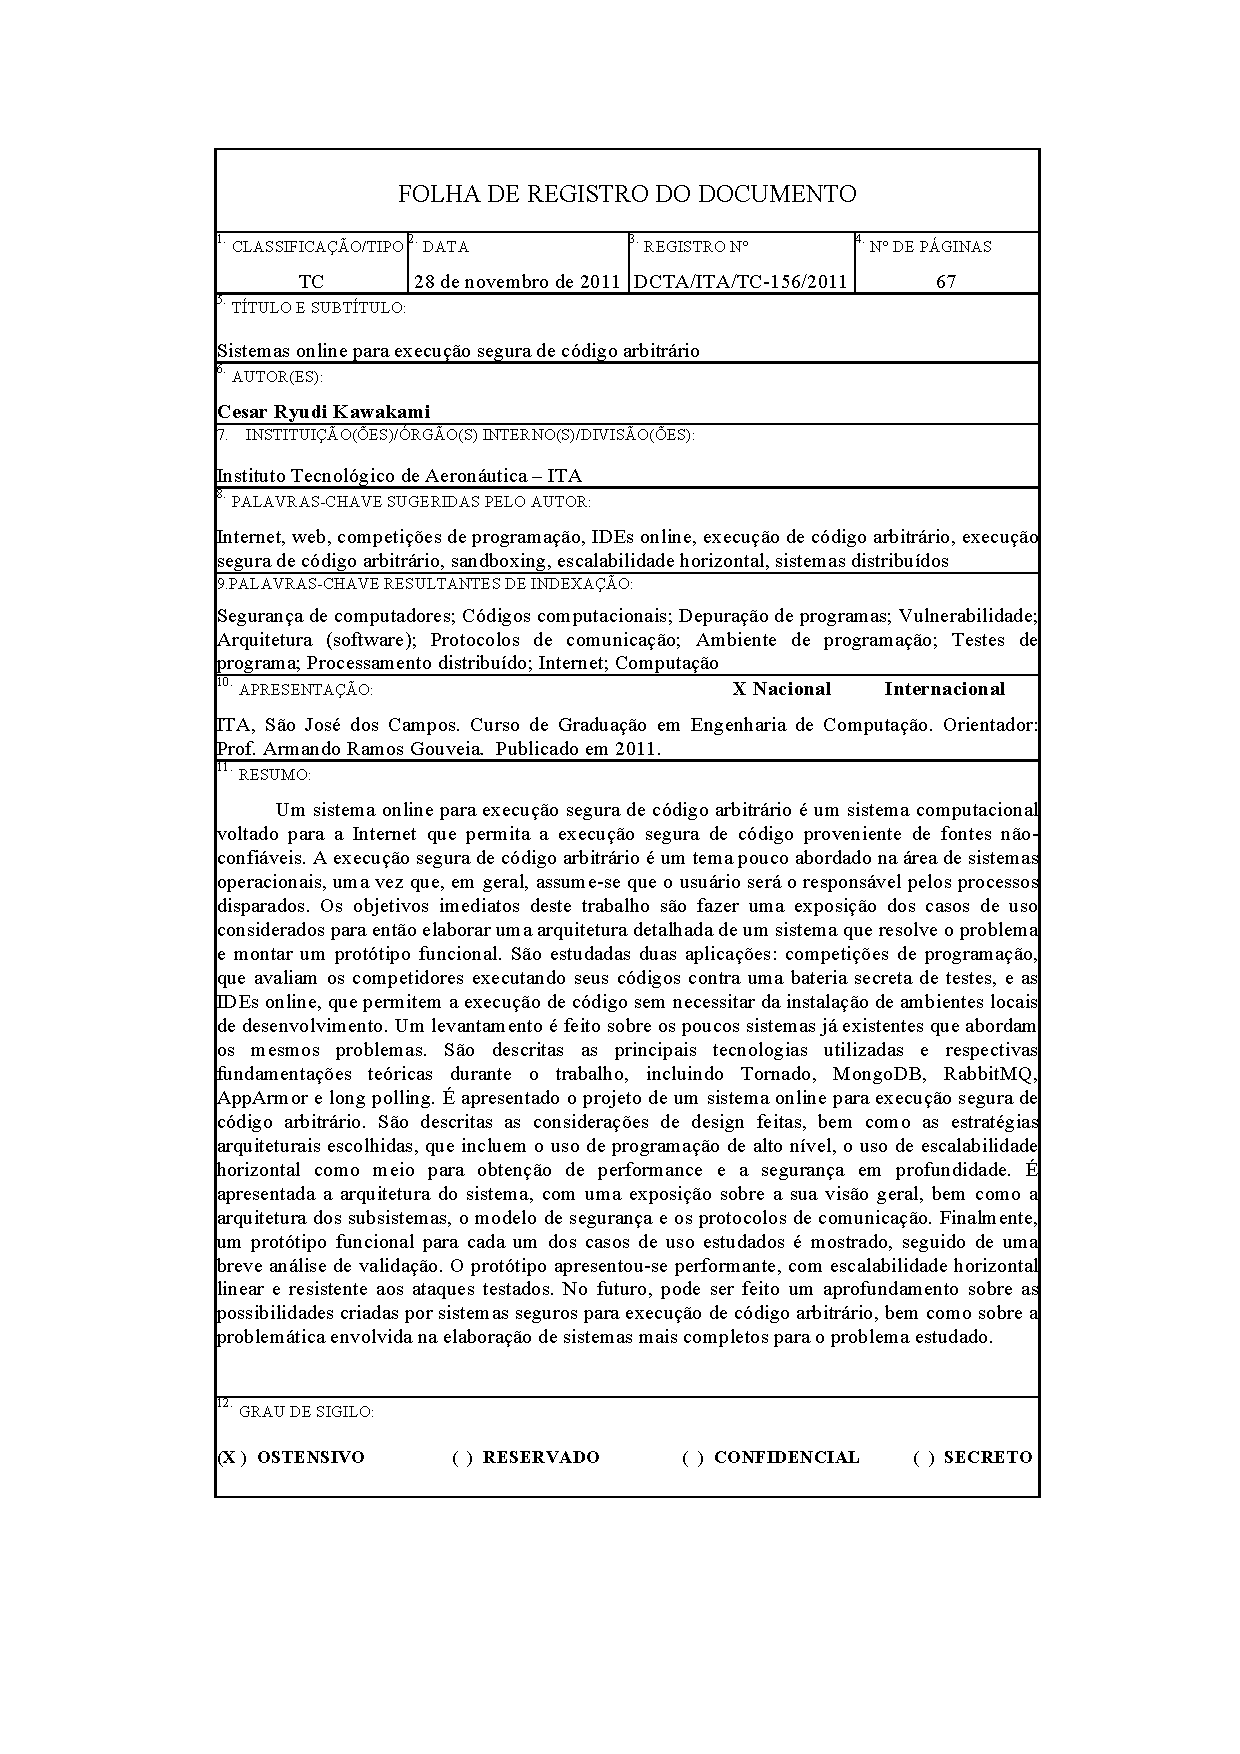
\includepdf{registro}

\bookmark[level=0, page=65]{Referências}

\bookmark[level=0, page=67]{Folha de Registro do Documento}

\end{document}
